%!TEX TS-program = xelatex
%!TEX encoding = UTF-8 Unicode

\documentclass{Dissertate}
\usepackage{siunitx}
%\usepackage[italian]{babel}
%\usepackage{latexsym}
\usepackage{booktabs}
\usepackage{etoolbox}
\AtBeginEnvironment{quote}{\singlespacing\small}
\newcommand{\numberset}{\mathbb}
%\usepackage{subfigure}
\usepackage{caption}
\captionsetup{singlelinecheck=true, justification=raggedright}
\usepackage[justification=centerfirst]{subcaption}
\usepackage{algorithm}
\usepackage{algpseudocode}
\usepackage{emptypage}
\usepackage[export]{adjustbox}
\renewcommand{\vec}[1]{\ensuremath{\boldsymbol{\mathit{#1}}}}

\let\tmp\oddsidemargin
\let\oddsidemargin\evensidemargin
\let\evensidemargin\tmp
\reversemarginpar

\begin{document}

% the front matter
%!TEX root = ../dissertation.tex
% Some details about the dissertation.
\title{Local Path Planning with Moving Obstacle Avoidance based on Adaptive MPC in ATLASCAR2}
\author{Alberto Franco}

%If you have one advisor
\advisor{Angelo Cenedese}

\committeeInternalOne{Vitor Santos}
\committeeInternalTwo{Person Inside Two}

%If you are coadvised
\coadvisorOne{Delightful Researcher}
\coadvisorTwo{Equally D. Researcher}
\committeeInternal{Person Inside}

% Everyone has an External committee member
\committeeExternal{Person Outside}

% ... about the degree.
\degree{Automation Engineering}
\degreeyear{2019}
\degreeterm{Spring}
\degreemonth{15$^{\text{th}}$ April}
\department{Information Engineering}


% \maketitle
% \copyrightpage
\frontmatter
\setstretch{\dnormalspacing}
 %\abstractpage
 %\tableofcontents
 %\authorlist
 %\listoffigures
 %\dedicationpage
 %\acknowledgments

% \doublespacing

% include each chapter...
\setcounter{chapter}{0}  % start chapter numbering at 0
\chapter{Introduction}
%\addcontentsline{toc}{chapter}{Introduction}
In robotic research, the problem of navigation is among the most important. Basically, all autonomous mobile robots need some kind of navigation abilities to perform, localization, motion planning and guidance \cite{Skoda:Thesis:2016}. In the present context, we focus on navigation as a process of planning a path of a mobile robot from its current position to a desired goal location, following the planned path, and avoiding any discovered obstacles along the way. The desired paths have to fulfill several conditions to ensure safety and feasibility of the navigation. Moreover, the paths can be also defined in terms of specifications; for example, short or smooth paths are usually more desirable than long and curved ones in every dynamic environments. 

Beyond the path planning, the navigation problem also involves reacting to changes of the environment model. Robots are required to move towards the target in a short time and avoid either static or dynamic obstacles observed by their sensors, which involves efficient path planning and valid obstacle avoidance. 

Research and development of Unmanned Ground Vehicles has been dominated by DARPA (Defense Advanced Research Projects Agency) and NASA (National Aeronautics and Space Administration). The DARPA initiative started with the development of the first mobile robot, Shakey, and also includes the Autonomous Land Vehicle and the DARPA Demo I1 Program. NASA sponsors the development of unmanned vehicles for planetary surface exploration, from the Jet Propulsion Laboratory Mars Rover to the most recent Mars Pathfinder. Recent UGV design and development has been enhanced to build UGVs capable of operating in Intelligent Vehicle Highway Systems \cite{Bai2015}.

Over the last decades, the development of Advanced Driver Assistance Systems has become a critical endeavor to attain different objectives: safety enhancement, mobility improvement, energy optimization and comfort \cite{Gruyer2017}. Much of the argument used in this discussion is based on the road mortality we see today. According to data from the World Health Organization, in 2013 there were about 1.25 million road deaths worldwide, and this number is expected to increase in the next decade \cite{world2015global}. Algorithms for autonomous navigation are increasingly robust and reliable and are starting to handle complex situations and decision problems.

According to Katrakazas \cite{Katrakazas2015}, local navigation is responsible for guiding the vehicle, that is, for the planning of the direction and speed to be taken, in a space close to the current position based on information exclusively obtained by the sensors on board. The guiding must be planned in such a way as to guarantee the displacement, from the current state to the objective, without collisions.

The algorithms we have developed at the LAR, follow a new and different approach for an advanced control strategy for autonomous navigation. The idea is that these methods do not replace the algorithms developed previously but are a valid alternative, so that depending on the situation, the vehicle can choose the best strategy to overcome obstacles or solve problems that can occur on the road that need a decision in real time.  Simulation results demonstrate and verify the feasibility and the usefulness of methods considering different scenarios.

In this introductory chapter, the ATLAS project is presented in more detail in section \ref{sec:ATLAS}, while examples of autonomous navigation projects are discussed later (section \ref{sec:autonomous_examples}). The context of the problem and the proposed solution of this thesis are carried out in section \ref{sec:context} while the organization of the document is discussed in section \ref{sec:outline}.
\section{ATLAS Project}\label{sec:ATLAS}
The ATLAS project was created in 2003 by the Group for Automation and Robotics from the Department of Mechanical Engineering at the University of Aveiro \cite{vsantos2010}. The objective of this project is to study and develop advanced sensors and active systems to promote the autonomous control of cars and other platforms. The first projects in the autonomous driving area focused on small scale models in controlled environments for participation in the National Robotics Festival (FNR) and in many other competitions winning some awards for the best performance (subsection \ref{sec:ATLASplatform}). The success and experience gained with these models allowed the evolution of the project for full-scale vehicles, where ATLASCAR (subsection \ref{sec:ATLASCAR}) in 2010 and ATLASCAR2 (subsection \ref{sec:ATLASCAR2}) in 2016 have been developed.

\subsection{ATLAS platforms}\label{sec:ATLASplatform}	
The first developed robot (Figure \ref{fig:modelosatlas1}) was based on an aluminum and wood structure. In this prototype only one camera was installed that pointed to a mirror to allow the complete visualization of the road in which the robot circulated. The traction movement was assured by a mechanical differential coupled to the rear wheels and the steering movement was given by a single front wheel. In order to create a model more similar to an ordinary car, the ATLAS group developed the ATLAS 2000 (Figure \ref{fig:modelosatlas2}) in scale (1:4), with which it managed to win the first autonomous driving competition of the FNR in 2006. After several improvements made in ATLAS 2000, in 2008 a new platform, ATLAS MV (Figure \ref{fig:modelosatlas3}) was created. This robot was designed on a smaller scale (1:5), with the intention of being lighter and faster. On board were installed a new steering system, hydraulic braking and an active perception unit. This robot allowed the conquest of new victories in the autonomus driving competitions.
\begin{figure}[!h]
	\centering
		\begin{minipage}[t]{0.32\textwidth}
			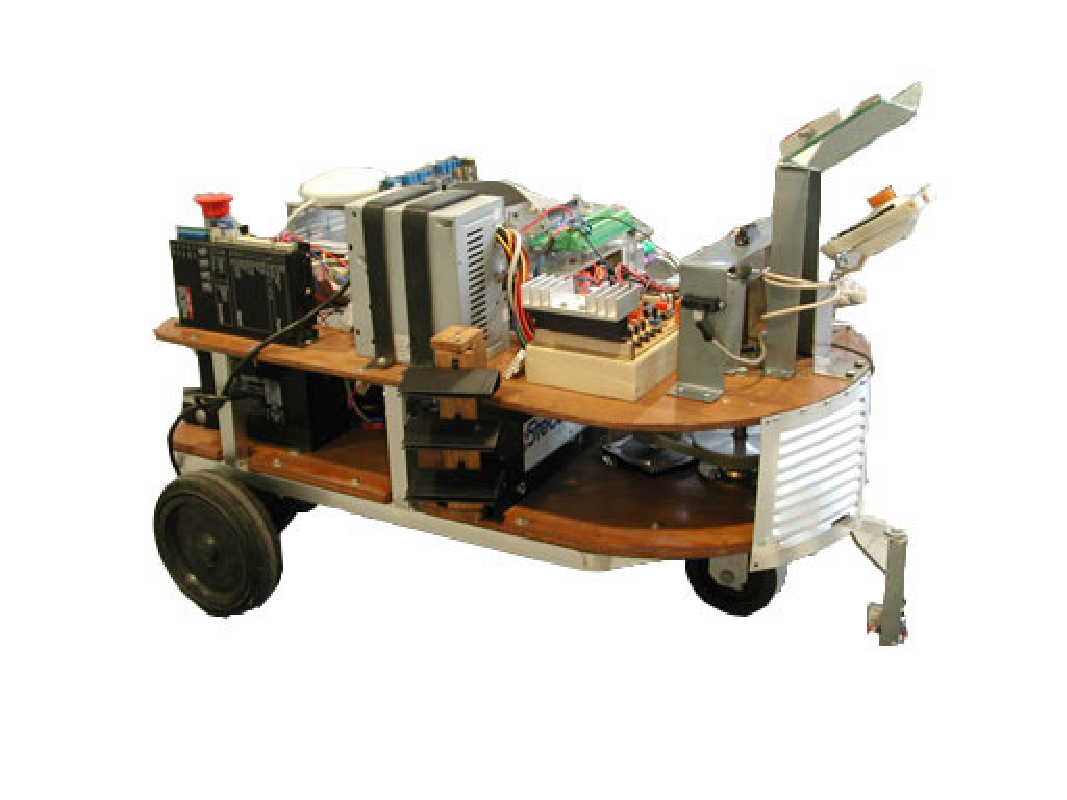
\includegraphics[width=\textwidth]{../figure/modelosatlas1.pdf}
			\subcaption{First ATLAS prototype.}
			\label{fig:modelosatlas1}
		\end{minipage}
		\begin{minipage}[t]{0.32\textwidth}
			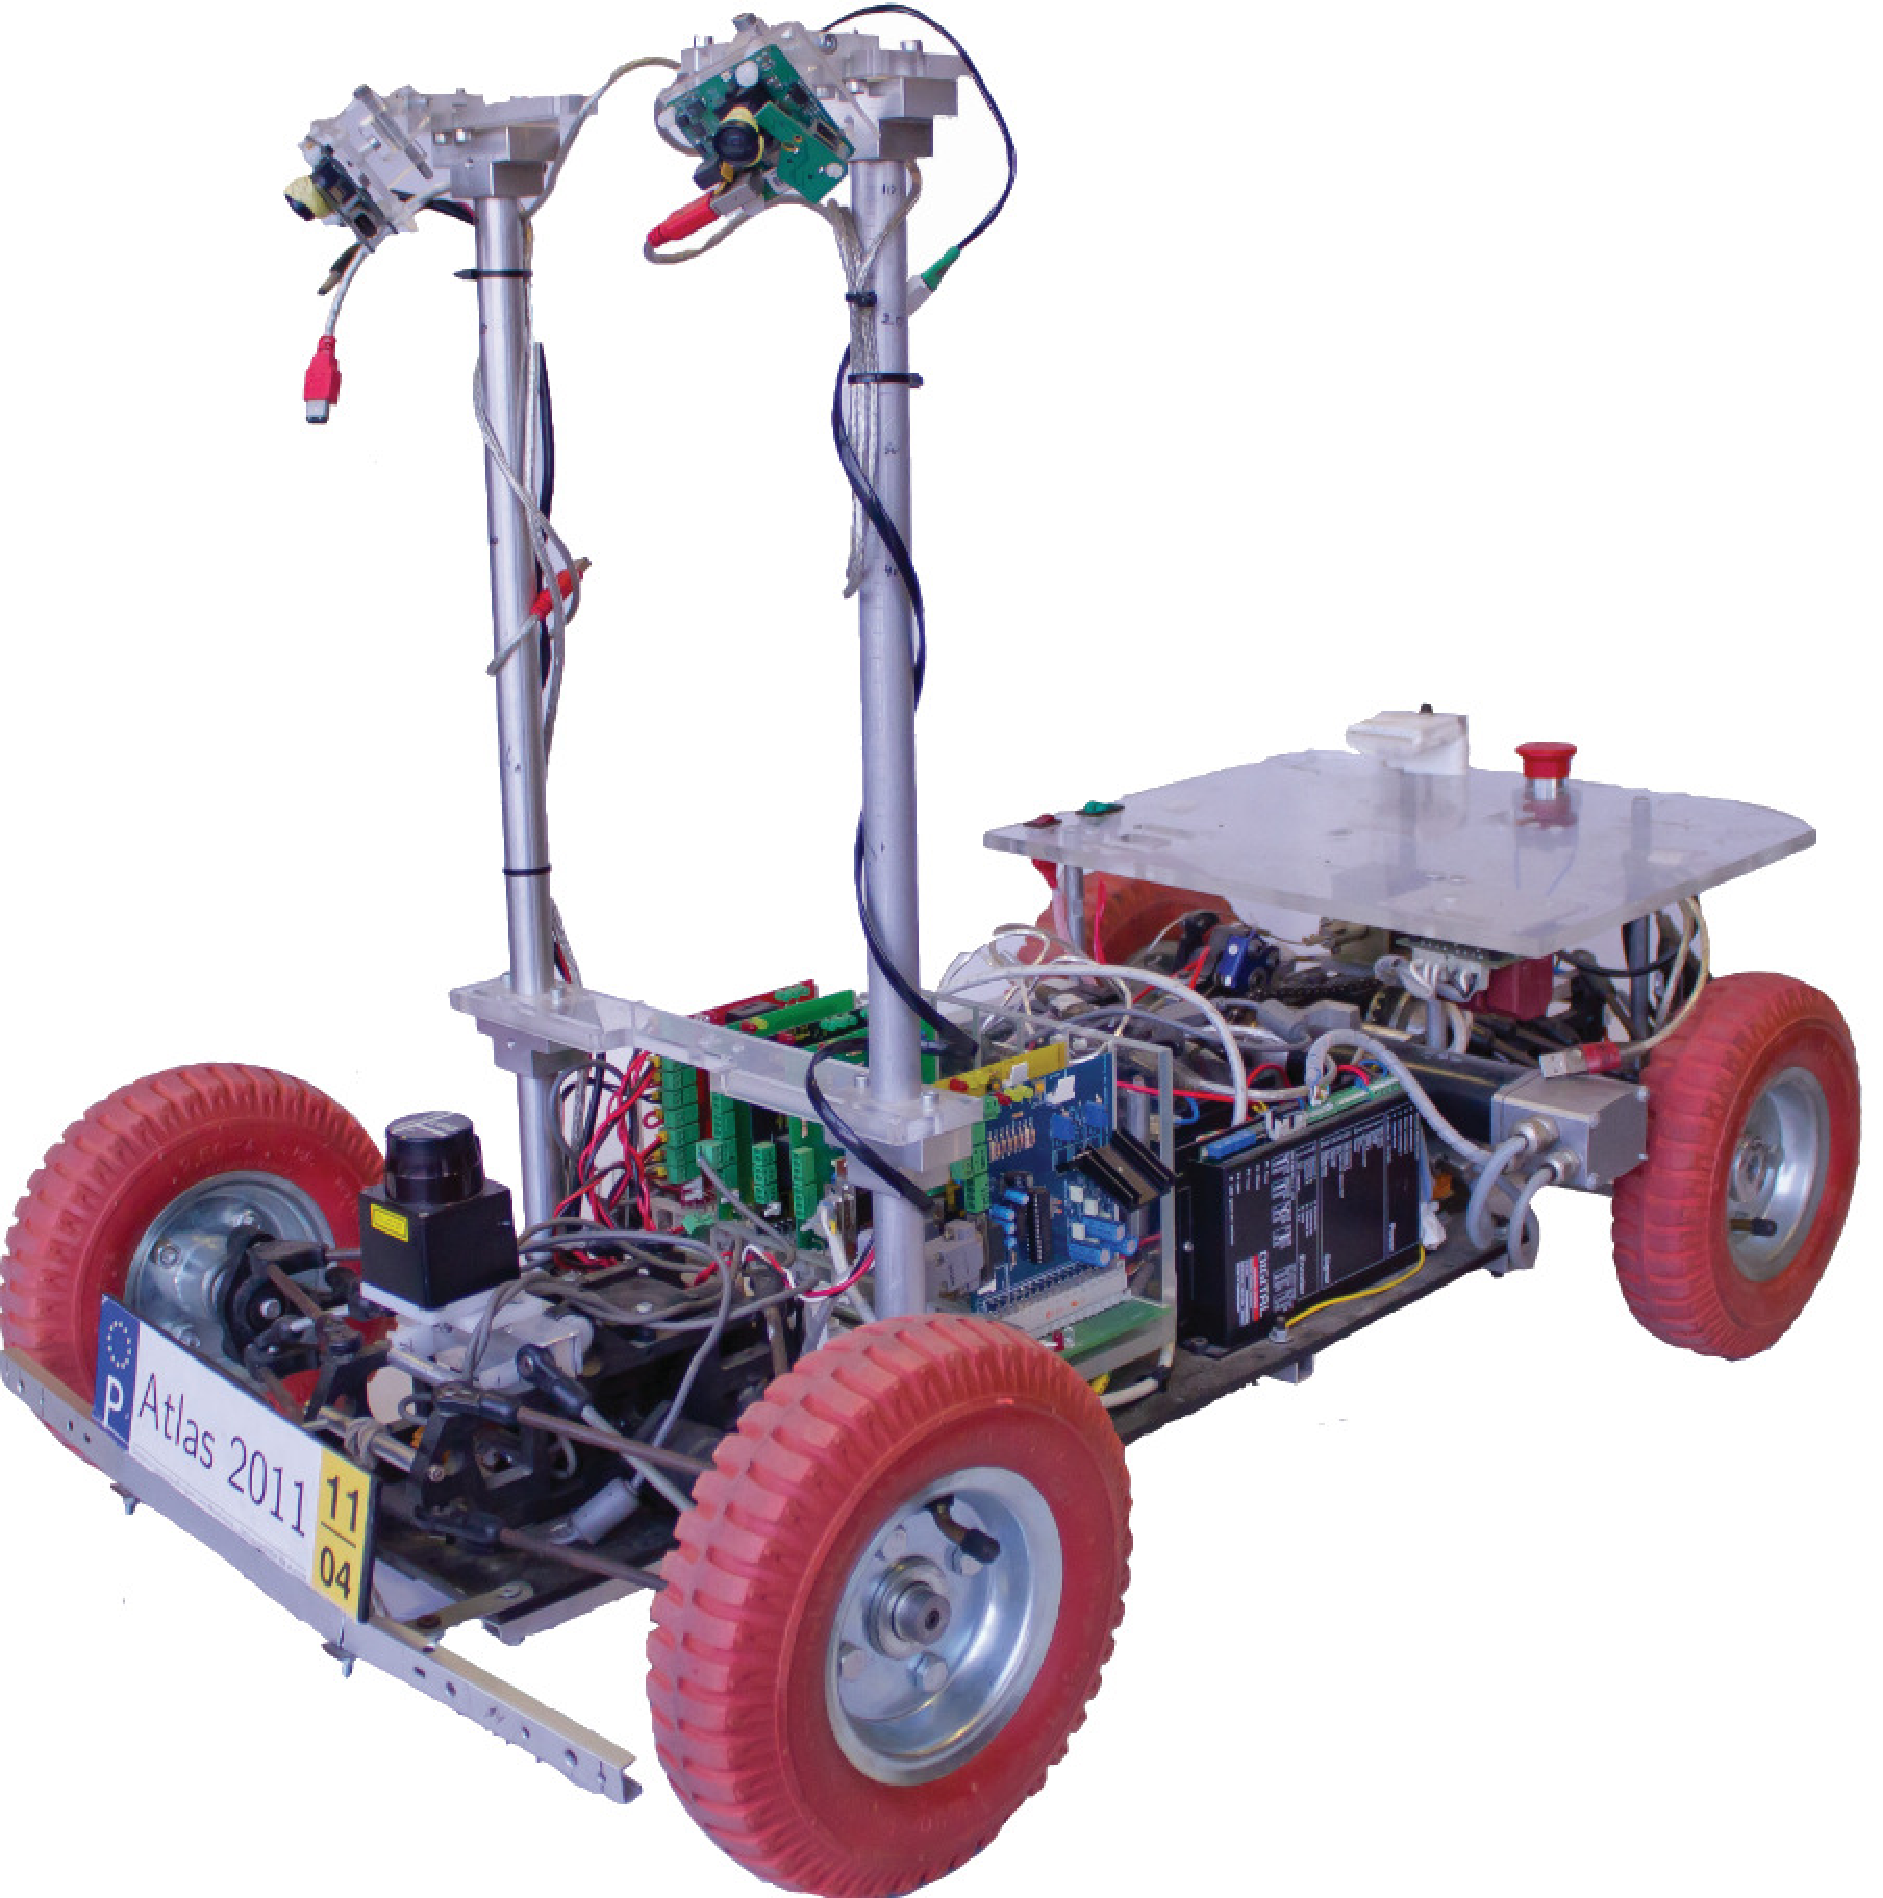
\includegraphics[width=\textwidth]{../figure/modelosatlas2.pdf}
			\subcaption{ATLAS 2000.}
			\label{fig:modelosatlas2}
		\end{minipage}
		\begin{minipage}[t]{0.32\textwidth}
			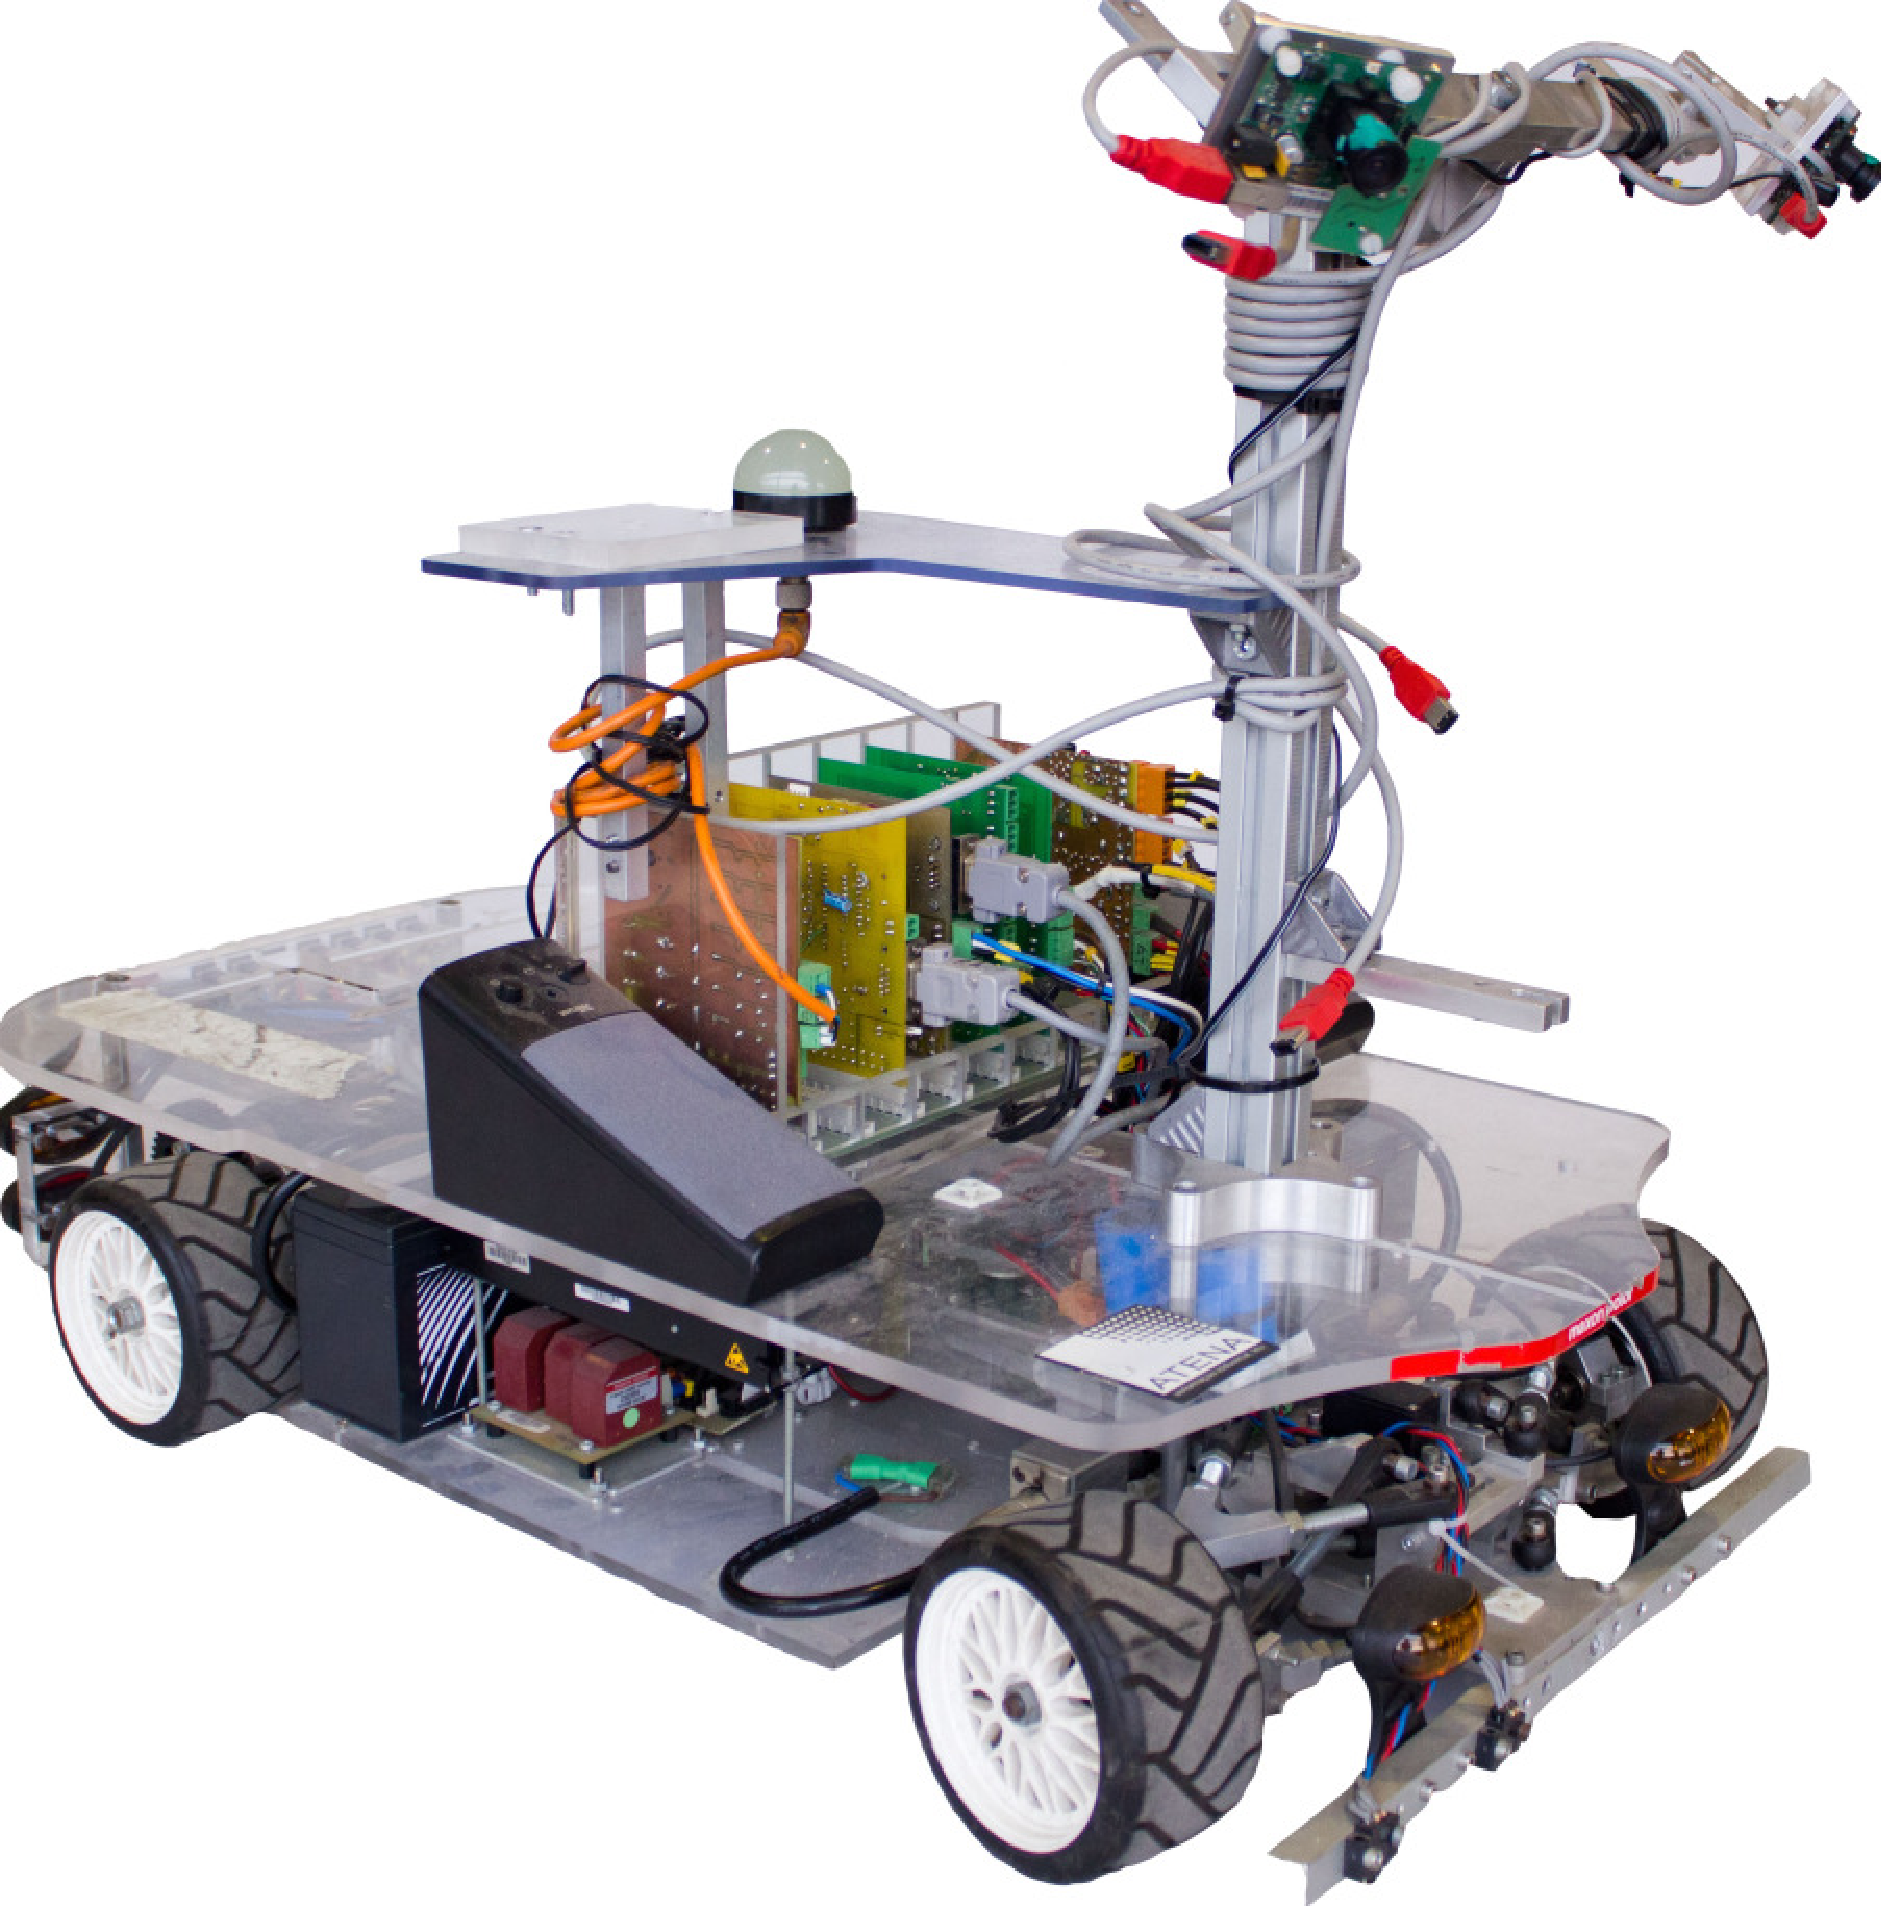
\includegraphics[width=\textwidth]{../figure/modelosatlas3.pdf}
			\subcaption{ATLAS MV.}
			\label{fig:modelosatlas3}
		\end{minipage}
		\caption{Some of the ATLAS project small scale platforms (adapted from \cite{Pereira2012}).}
		\label{fig:modelosatlas}
\end{figure}

\subsection{ATLASCAR}\label{sec:ATLASCAR}
Driven by the positive results achieved with scale models and years of navigation experience in controlled environments, in 2010 the Group of Automation and Robotics decided to invest in a large-scale project, ATLASCAR (Figure \ref{fig:atlascar1}). The vehicle used for this project was a Ford Escort Station Wagon of 1998 powered by a gasoline internal combustion engine, in which several sensors, processing units and actuators were installed. On-board sensors processed data collected from the vehicle and its surroundings, with different LIDARs for obstacle detection and environmental reconstruction, pedestrian detection cameras and a Global Navigation Satellite System (GNSS) for location and route planning. After passing through the processing units, these data were sent to the actuators that allowed the movement and execution of the maneuvers in a completely autonomous way on the part of the vehicle. To power all the equipment, a Uninterruptible Power Supply (UPS) was used, loaded from an auxiliary alternator. During this project, many works were developed in the Laboratory for Automation and Robotics, many of which produced master thesis. For example, in 2014 Cabral de Azevedo \cite{Azevedo2014} developed a module to detect pedestrians using sensory fusion of LIDAR and vision data while in 2016 Vieira da Silva \cite{Silva2016} created a multisensory calibration module that was exported to subsequent projects.
\begin{figure}[!h]
	\centering
	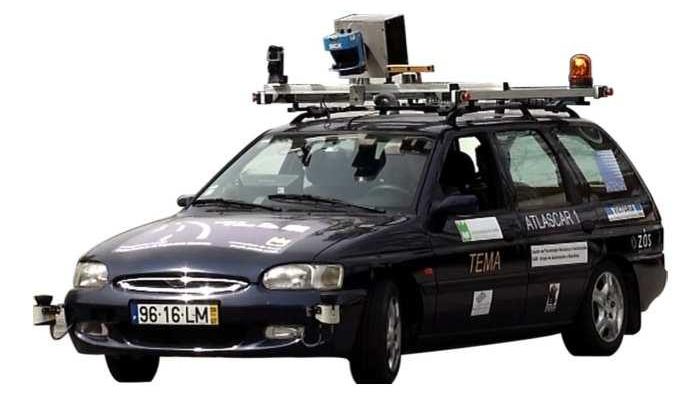
\includegraphics[width=\textwidth]{../figure/atlascar1.jpg}
	\caption{The car used in ATLASCAR, based on Ford Escort Station Wagon of 1998 (adapted from \cite{Pereira2012}).}
	\label{fig:atlascar1}
\end{figure}

\subsection{ATLASCAR2}\label{sec:ATLASCAR2}
Given the different limits, to continue the project, in 2016, a new vehicle was acquired: ATLASCAR2 (Figure \ref{fig:atlascar2}). This time it was chosen as a platform
an electric car, a Mitsubishi iMiEV, with an autonomy range of \SI{100}{km}. The fact that the vehicle is electric allows to use the energy stored in the batteries, making it easier to power the sensors installed. In fact, despite the short time of existence, 3 LIDARs, a camera, inclinometry sensors and a GNSS unit are already installed on the ATLASCAR2. Many of these sensors were transferred from ATLASCAR to this project during the work of Madureira Correia \cite{Madureira2017} in 2017, where a module for detecting free space around the car was also developed while in 2018 Ricardo Silva \cite{Ricardo:Thesis:2018} created a local navigation module for driver assistance in the immediate decision making, identifing a solution based on a multiple hypothesis approach.
\begin{figure}[!h]
	\centering
	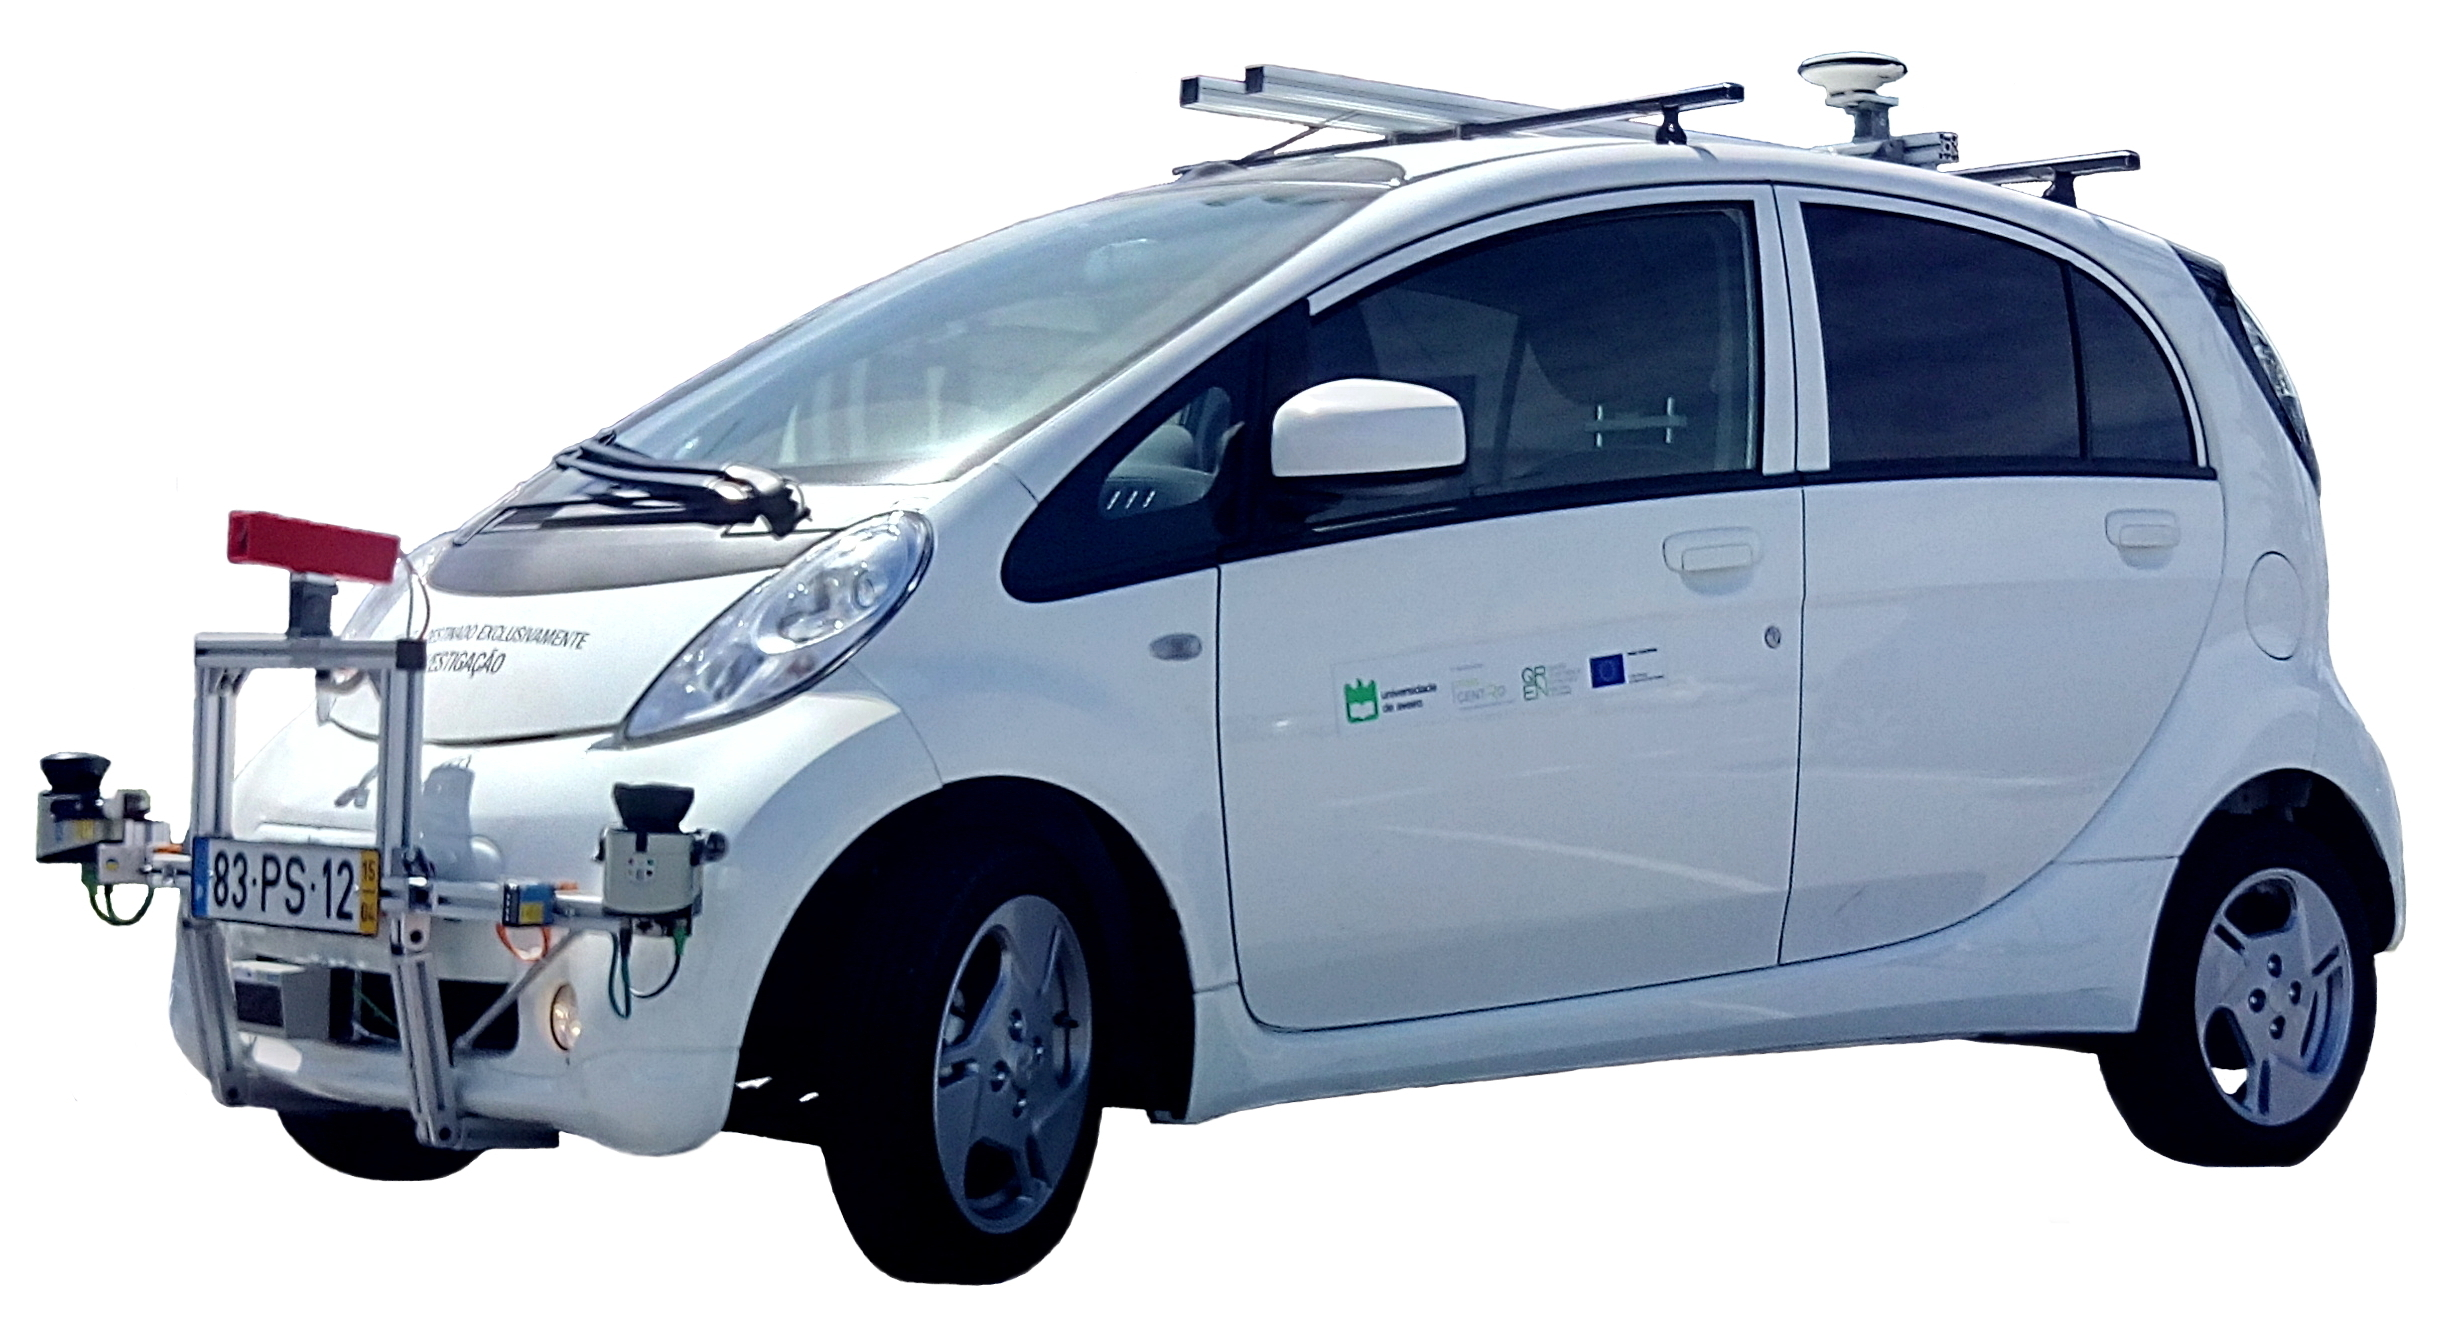
\includegraphics[width=\textwidth]{../figure/atlascar2.jpg}
	\caption{The vehicle used in ATLASCAR2, based on an electric car, a Mitsubishi iMiEV of 2015 (adapted from \cite{Ricardo:Thesis:2018}).}
	\label{fig:atlascar2}
\end{figure}

\section{Autonomous Cars}\label{sec:autonomous_examples}
The legal definition of autonomous vehicle in the District of Columbia code is:
\begin{quotation}
	\itshape ''Autonomous vehicle'' means a vehicle capable of navigating District roadways and interpreting traffic-control devices without a driver actively operating any of the vehicle's control systems. The term ''autonomous vehicle'' excludes a motor vehicle enabled with active safety systems or driver-assistance systems, including systems to provide electronic blind-spot assistance, crash avoidance, emergency braking, parking assistance, adaptive cruise control (ACC), lane-keep assistance (LKA), lane-departure warning, or traffic-jam and queuing assistance, unless the system alone or in combination with other systems enables the vehicle on which the technology is installed to drive without active control or monitoring by a human operator. 
\end{quotation}

The modern automobile companies keep coming up with newer autonomous features in their recent models. Technological advancements seen every day in areas like information technology, communication, data analysis and storage etc. is not exclusive to these areas alone. The realm of autonomous cars is also progressing at a rapid rate these days \cite{Bimbraw2015}. Google's development of self-driving technology began in January 2009. The initial objective of the project was to develop a car able to navigate on highways with minimal human intervention. In December 2016, the unit was renamed Waymo; this name derived from its mission, "a new way forward in mobility". Waymo moved to further test its cars on public roads after becoming its own subsidiary.
\begin{figure}[!h]
	\centering
	\begin{minipage}[t]{0.65\textwidth}
		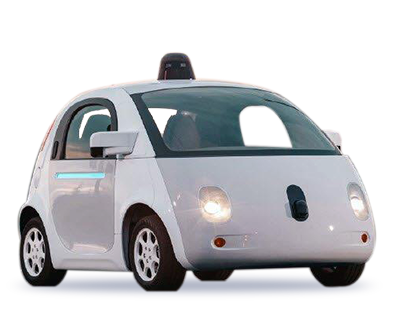
\includegraphics[width=\textwidth]{../figure/veiculos0.png}
		\subcaption{Google's Firefly self-driving prototype in 2015 (adapted from \cite{waymoh}).}
		\label{fig:veiculos0}
	\end{minipage}
	\begin{minipage}[t]{0.65\textwidth}
		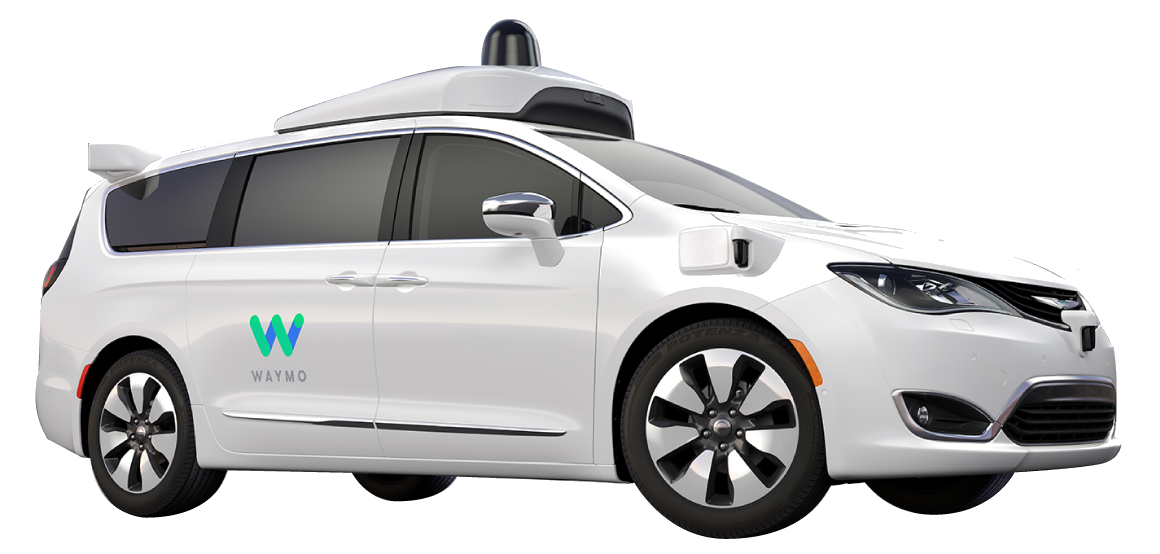
\includegraphics[width=\textwidth]{../figure/veiculos1.png}
		\subcaption{Waymo Chrysler Pacifica Hybrid self-driving prototype in 2017 (adapted from \cite{waymoh}).}
		\label{fig:veiculos1}
	\end{minipage}
	\caption{Some of the Waymo/Google prototypes tested across multiple locations in the Unided States in recent years.}
	\label{fig:waymo}
\end{figure}

Waymo uses LIDAR which sends out millions of laser beams per second to build up a detailed picture of the world all 360 degrees around it. It also uses radar to detect how far away objects are and their speed and high-resolution cameras detect visual information like whether a traffic signal is red or green. It then combines all that data to understand the world around it and predict what those things might do next. It can do that for things up to three football fields away. Based on all this information, Waymo's software determines the exact trajectory, speed, lane and steering maneuvers needed to progress along this route safely \cite{waymoh} \cite{waymot}.

With the advances in autonomous technology, VIAC or VisLab Intercontinental Autonomous Challenge was one of the major competitions which led to improvements in the testing and analysis of autonomous vehicles and robotics. It was a 13,000 kilometers trip, nearly three months from Parma, Italy to Shanghai, China from July 20, 2010 to October 28, 2010. It involved four autonomous vehicles with negligible human intervention and high level of autonomy \cite{Broggi2010}. One of VisLab's advanced autonomous car, BRAiVE (Figure \ref{fig:veiculos4}), drove in downtown Parma on July 12th, 2013. It successfully navigated narrow rural roads, crosswalks, traffic lights, pedestrian areas, roundabouts and artificial hazards. It was a pioneer in the field of vehicular robotics, since it was totally autonomous \cite{Broggi2013}.
\begin{figure}[!h]
	\centering
	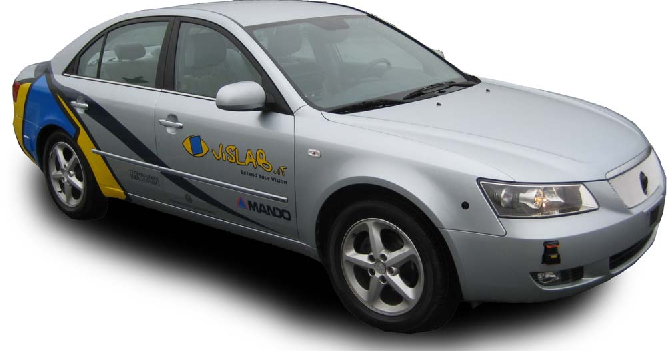
\includegraphics[width=0.65\textwidth]{../figure/veiculos4.png}
	\caption{BRAiVE prototype developted by VisLab, based on a Hyundai Sonata (adapted from \cite{Broggi2013}).}
	\label{fig:veiculos4}
\end{figure}

Another example of autonomous system is Navya, a robotically driven electric shuttle which operates at a maximum speed of 25 kilometers per hour. Made by Induct Technology, France, it can accommodate 15 passengers. It uses four LIDAR units and stereoscopic optical cameras, and it does not
require any road modifications. Its LIDAR unit and
optical cameras help in generating a real-time three dimensional map of the surroundings. It is being successfully tested at various universities across Switzerland, England and Singapore \cite{Zhang2014}.

\begin{figure}[!h]
	\centering
	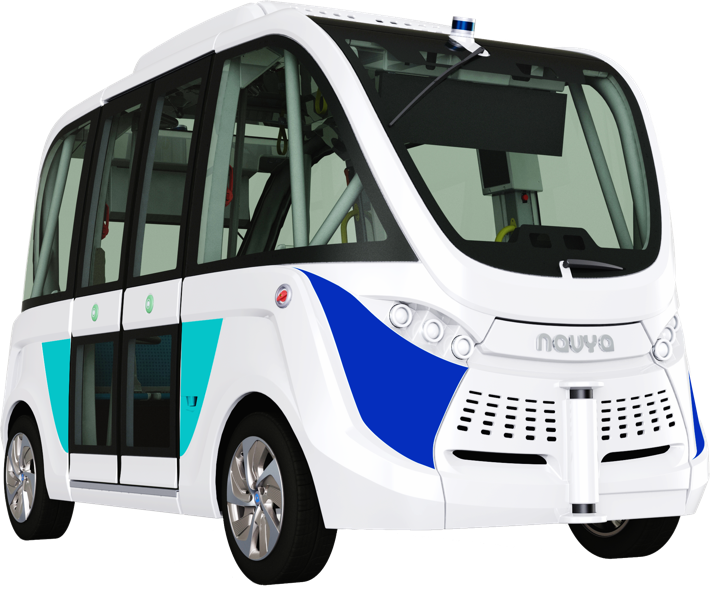
\includegraphics[width=0.6\textwidth]{../figure/veiculos5.png}
	\caption{Navya Shuttle developted in 2016 by Navya Group in France.}
	\label{fig:veiculos5}
\end{figure}

\section{Context of the Problem and Proposed Approach}\label{sec:context}
Dynamic environments pose several added difficulties to the motion planning problem. The dynamics of the ATLASCAR2 must be taken into account, and there are limitations due to the sensors range and uncertainty in measurements, that must be reflected on the motion plan. Besides it, a motion plan must incorporate time restrictions, meaning the vehicle will require a certain amount of time to accomplish a task. For example, when crossing a road, the ATLASCAR2 must do it fast enough to avoid incoming cars. The proposed algorithms were studied for the ATLASCAR2 project in which the group for Robotics and Automation at the University of Aveiro has setup and adapted a common commercial electric vehicle to provide a versatile  framework  to  develop  studies  and  research \cite{vsantos2010} \cite{vsantos2019}. The fact that the vehicle is electric allows to use the energy stored in the batteries, making it easier to power the sensors installed. In fact, the ATLACAR2 is equipped with sensors, such as lidar, that measure the distance to obstacles in front and around the vehicle. The obstacles can be static, such as a large pothole, or moving, such as a moving vehicle on the same or a nearby lane. The most common maneuver from the driver is to temporarily move to another lane, drive past the obstacle, and move back to the original lane afterward. In this case, we want to design an obstacle avoidance system that moves the ATLASCAR2 around  moving obstacles in the lane using throttle and steering angle. This system uses an adaptive Model Predictive Controller that updates both the predictive model and the mixed input/output constraints at each control interval. Moreover we want to develop a lane-keeping assist system for the vehicle: it has a sensor, such as camera or laser, that measures the lateral deviation and relative yaw angle between the centerline of a lane and the ATLASCAR2; it also measures the current lane curvature and its derivative. Depending on the curve length that the sensor can view, the curvature in front of the vehicle can be calculated from the current curvature and its derivative. This system keeps the autonomous car travelling along the centerline of the lanes on the road by adjusting the front steering angle. The goal for lane keeping control is to drive both lateral deviation and relative yaw angle close to zero.

\section{Thesis Outline}\label{sec:outline}

In this section, we outline the thesis organization: 

Chapter 1 is used to introduce the thesis focus areas of autonomous vehicle technology. In particular the ATLAS project and examples of autonomous navigation projects are presented. Moreover the context of the problem and the objectives to be achieved are carried out.

Chapter 2 




\cleardoublepage
\chapter{Literature Review}
\cleardoublepage
\chapter{Model Predictive Control}

In this chapter, the theory of Model Predictive Control is discussed in detail to highlight working principle. In particular for this work we used an advanced control strategy based on this paradigm called Adaptive MPC that uses a fixed model structure, but allows the model parameters to evolve with the time.

\section{Generic Model Predictive Control problem}
Model Predictive Control (MPC), also known as Moving Horizon Control (MHC) or Receding Horizon Control (RHC), is a popular method for the control of slow dynamical systems, to generate the required
control inputs that are calculated at each sampling instance $k$, using the current state as initial
conditions to solve a finite optimal control problem. Some of the advantages of using MPC are:
\begin{itemize}
\item the ability to handle unstable, time variable, non-minimum phase systems;
\item robustness feature with the uncertainties in the nonlinear systems;
\item built in feed-forward control to handle disturbances in the processes;
\item enhanced tuning features to achieve the best response including transient responses;
\item the possibility to introduce constraints in a natural form;
\item if the references are known in advance, they can be used in order to optimize the reference tracking.
\end{itemize}


The methodology of all the controllers belonging to the MPC family is characterized by the following strategy, represented in Figure \ref{fig:mpc_theory}. The future outputs for a  determined horizon, called  the  prediction horizon, are predicted at each instant $k$ using the process model. These predicted outputs depend on the known values up to instant $k$ (past inputs and outputs) and on the future control signals which are those to be sent to the system and calculated. The set of future control signals is calculated by optimizing a determined criterion to keep the process as close as possible to the reference trajectory. This criterion usually takes the form of a quadratic function of the errors between the predicted output signal and the predicted reference trajectory. The control effort is included in the objective function in most
cases. An explicit solution can be obtained if the criterion is quadratic, the model is linear, and there are no constraints; otherwise an iterative
optimization method has to be used. Some assumptions about the structure of the future control law are also made in some cases, such as that it will be constant from a given instant. Only the current control signal is send to the process. At the next sampling instant the measured output is evaluated and the sequence is repeated and all the steps brought up to date. Thus the predicted control input is then calculated using the receding horizon concept.
\begin{figure}[!h]
	\centering
	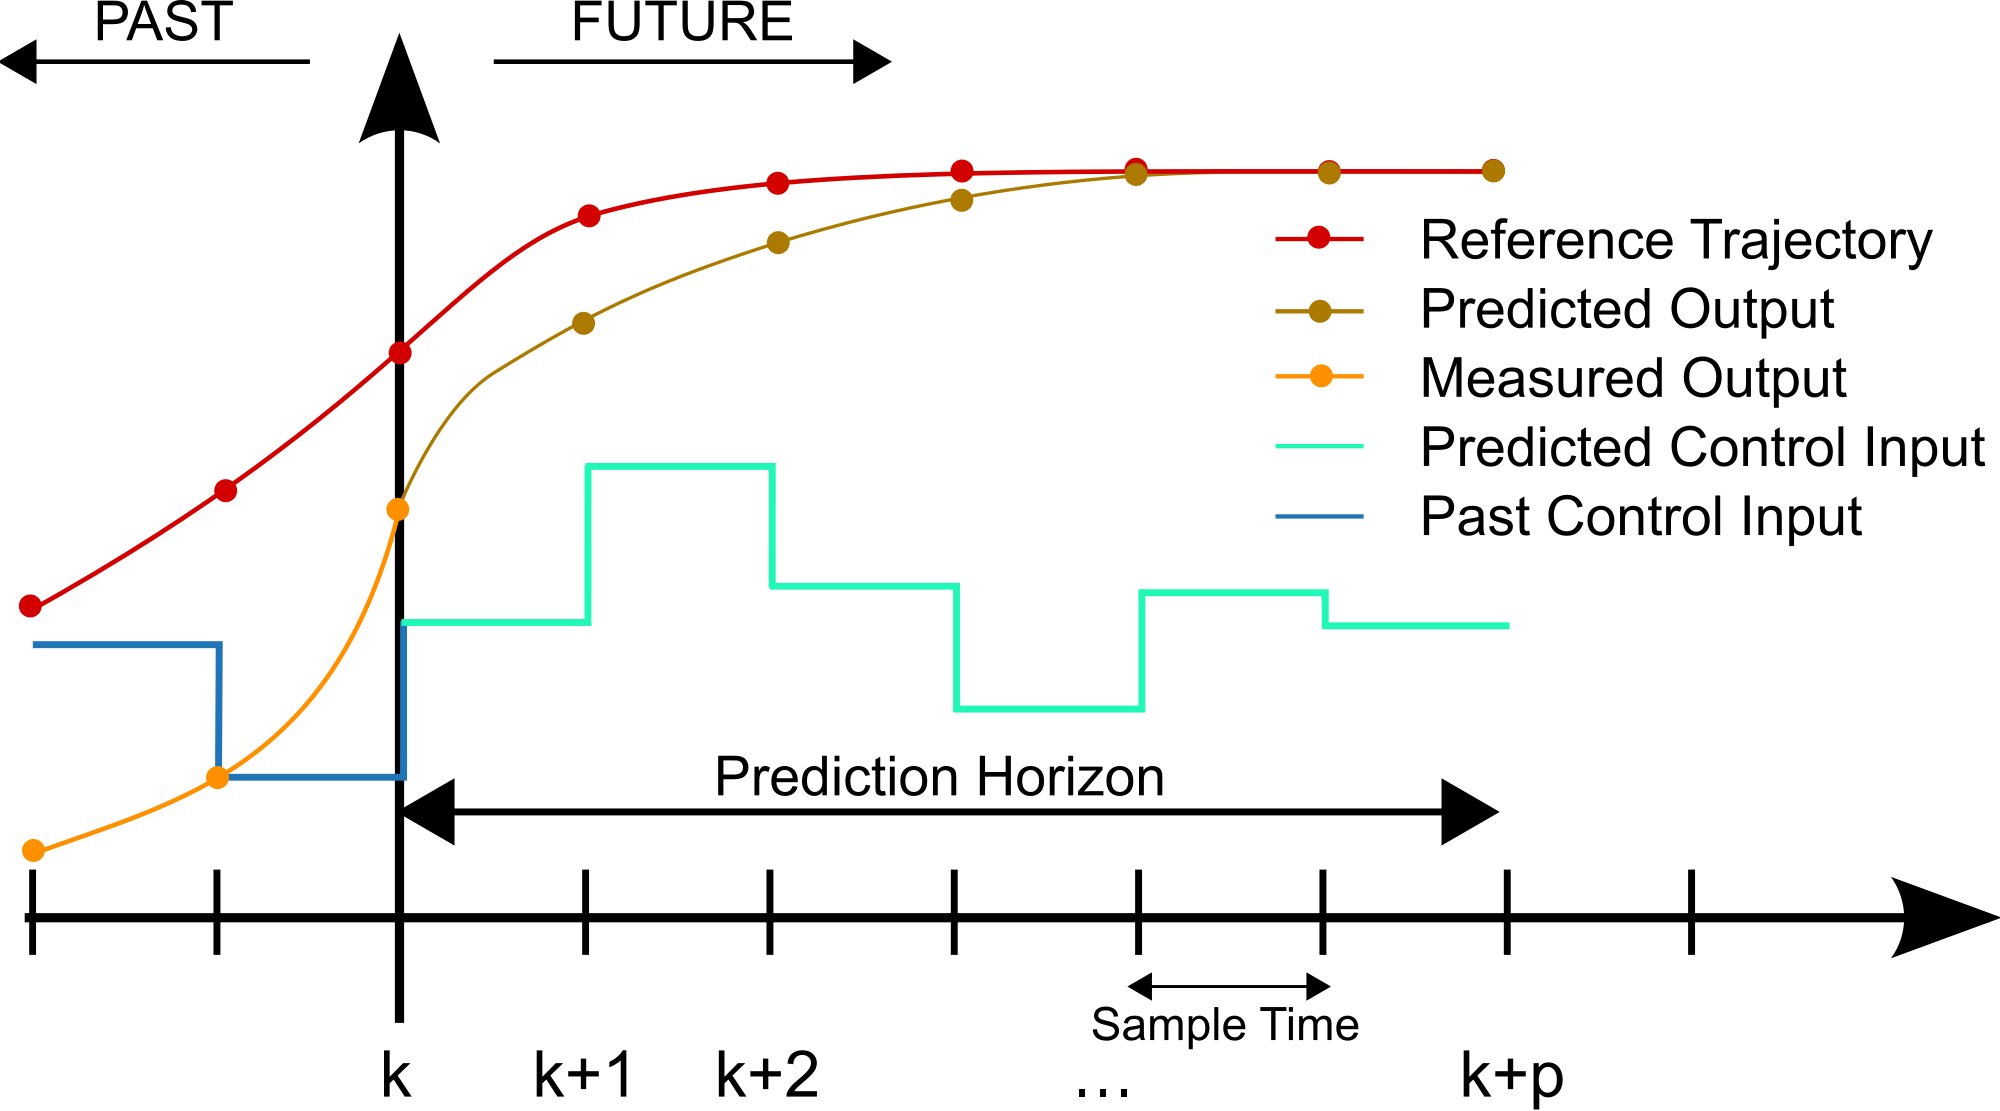
\includegraphics[width=\textwidth]{../figure/mpc_theory.png}
	\caption{A discrete Model Predictive Control scheme adapted from \cite{mpctoolbox}.}
	\label{fig:mpc_theory}
\end{figure}

MPC is typically formulated in the state space. For a given discrete linear time-invariant (LTI) system:
\begin{equation}
\label{eqn:MPC_plant_discrete}
\vec{x}(k+1)=\vec{A}\vec{x}(k)+ \vec{B} \vec{u}(k)
\end{equation}
where $\vec{x}(k)\in\mathbb{R}^n$, $\vec{u}(k)\in\mathbb{R}^m$ are the state and the input, respectively. The central idea in the Model Predictive Control is to minimize some cost function, while still ensuring that some constraints are fulfilled. The generic MPC problem can be written as follows:
\begin{equation}
\label{eqn:MPC_optimization}
\begin{aligned}
& \underset{\textbf{u}}{\text{minimize}}
& & J(\vec{x}(k), \textbf{u}) \\
& \text{subject to}
& & \vec{x}_{k+i+1} = \vec{A}\vec{x}_{k+i}+ \vec{B} \vec{u}_{k+i}\quad\forall i=0,\dots N-1;\\
& & & \vec{x}_{k+i}\in \mathbb{X}\quad\forall i=0,\dots N-1;\\
& & & \vec{u}_{k+i}\in \mathbb{U}\quad\forall i=0,\dots N-1;\\  
& & & \vec{x}_{k+N}\in \mathbb{X}_f;\quad\vec{x}_k = \vec{x}(k).
\end{aligned}
\end{equation}
where $\textbf{u}=(\vec{u}_k,\dots,\vec{u}_{k+N-1})$ is a sequence of control inputs, $\vec{x}_{k+i}$ is the state at time $k+i$ as predicted at time $k$, and $N$ is the prediction horizon. The sets $\mathbb{X}\in\mathbb{R}^n$ and $\mathbb{U}\in\mathbb{R}^m$ define the constraints on the state and the input, respectively. Finally, the set $\mathbb{X}_f\subseteq\mathbb{X}$ defines the terminal constraint on the state. If we consider a regulation problem, the system \ref{eqn:MPC_plant_discrete} should be steered to the origin and the cost function $J(\vec{x}(k), \textbf{u})$ could be in a quadratic form as follows:
\begin{equation}
\label{eqn:MPC_cost_function_regulation}
	J(\vec{x}(k), \textbf{u}) = \vec{x}^\intercal_{k+N}\vec{P}_f\vec{x}_{k+N}+\sum_{i=1}^{N}\vec{x}^\intercal_{k+i}\vec{Q}\vec{x}_{k+i}+\vec{u}_{k+i}^\intercal\vec{R}\vec{u}_{k+i}
\end{equation}
where $\vec{P}_f,\vec{Q}\geq0$ (positive semi-definite) and $\vec{R}>0$ (positive definite) are weighting matrices.

Instead if we consider a servo problem, like tracking of a reference signal, the cost function is changed as follows:
\begin{equation}
\label{eqn:MPC_cost_function_servo}
\begin{aligned}
J(\vec{x}(k), \textbf{u})=& (\vec{x}_{k+N}-\vec{x}^\text{ref}_{k+N})^\intercal\vec{P}_f(\vec{x}_{k+N}-\vec{x}^\text{ref}_{k+N})\\
&+\sum_{i=1}^{N}(\vec{x}_{k+i}-\vec{x}^\text{ref}_{k+i})^\intercal\vec{Q}(\vec{x}_{k+i}-\vec{x}^\text{ref}_{k+i})+\vec{u}_{k+i}^\intercal\vec{R}\vec{u}_{k+i}
\end{aligned}
\end{equation}
where $\vec{x}^\text{ref}_{k+i}$, $\vec{x}^\text{ref}_{k+N}$ describe the reference trajectory. The standard MPC algorithm can be summarized by the following steps:
\begin{algorithm}%[b]
	\caption{Basic Model Predictive Control loop}
	\small
	\begin{algorithmic}[1]
		\State Measure the current state $\vec{x}(k)$;
		\State Solve the optimization problem \ref{eqn:MPC_optimization} with $\vec{x}(k)$ as initial state, where $\vec{u}(k)$ is calculated;
		\State Apply the first control of the optimal control sequence;
		\State Wait one sampling time and repeat steps 1-3;
	\end{algorithmic}
	\label{alg:rightOvertaking}
\end{algorithm}

An MPC has many strengths. Given that the model is discrete and linear it handles multivariable problems very well. Also mathematical convexity is an important part of the resulting problem formulation of an MPC. In fact there exists efficient solvers for convex optimization problems but it is therefore desirable that the MPC problem \ref{eqn:MPC_optimization} is convex which is ensured if:
\begin{enumerate}
\item the cost function is convex;
\item the prediction model is linear;
\item the constraint sets $\mathbb{X}, \mathbb{U}$ are convex.	
\end{enumerate}	
The optimization handles actuator constraints and state constraints naturally in the optimization which allows for
the process to be operated much closer to the hard constraints, which improves control performance and efficiency. Because of its predictive nature it is able to solve a variety of problems and handle disturbances smoothly.

\subsection{Tuning Parameters}
The two most important parameters to tune in order to satisfy the control objectives are the diagonal matrices $\vec{Q}$ and $\vec{R}$ that can be used to weight the system state matrix and the control inputs respectively. The response of the system that is too slow can be influenced by adding high weighting values in the $\vec{Q}$ matrix, whereas the control gains are damped with high weighing values in the $\vec{R}$ matrix. Find an optimal trade-off is a fundamental aspect for the constroller behaviour.

\subsection{Stability of MPC controller}
A limited horizon on the MPC problem affects the stability of the controllers; in order to avoid this problem it is possible to set an infinite horizon, impose end point constraints, terminal cost function or use other techniques. To obtain a stable controller, the parameters to tune are: the terminal cost, prediction horizon and constraints. Also the weights on the cost function can be tuned to ensure a stabilizing solution.

\subsection{Robustness}
If the stability can be guaranteed and the performance specifications are met with respect to a certain set of uncertainties, the system is said to be robust; in particular a controller with this property has to ensure that the constraints are never violated for any admissible disturbance realization. The uncertainties in a system are due to external disturbances, measurement noise, inaccurate values of the model parameters, non-linearities etc...
The most common type of uncertainties considered in the literature is additive disturbance because usually the current state of the system can be measured hence there is no noise in the measurements.

\section{Adaptive Model Predictive Control}
We understood that Model Predictive Control is an advanced method that predicts future behavior using a linear-time-invariant (LTI) dynamic model. These predictions are not exact and a good strategy is to make MPC insensitive to prediction errors. If the plant is strongly nonlinear or its characteristics vary dramatically with time, MPC performance might become unacceptable because LTI prediction accuracy degrade \cite{mpctoolbox}. A method that can address this degradation by adapting the prediction model for changing operating conditions is called Adaptive MPC: this control strategy uses a fixed model structure, but allows the model parameters to evolve with time. Ideally, whenever the controller requires a prediction, it uses a model appropriate for the current conditions. At each control interval, the adaptive MPC controller updates the plant model and nominal conditions. Once updated, the model and conditions remain constant over the prediction horizon. The plant model used as the basis for the adaptive MPC must be an LTI discrete-time, state-space model with a structure as follows:
\begin{equation}
\label{eqn:Adaptive_MPC_plant_discrete}
\begin{aligned}
\vec{x}(k+1)&=\vec{A}\vec{x}(k)+ \vec{B}_u \vec{u}(k)+\vec{B}_v \vec{v}(k)+\vec{B}_d \vec{d}(k)\\
\vec{y}(k)&=\vec{C}\vec{x}(k) + \vec{D}_v \vec{v}(k)+ \vec{D}_d \vec{d}(k)
\end{aligned}
\end{equation}
where the matrices \vec{A}, $\vec{B}_u$, $\vec{B}_v$, $\vec{B}_d$, \vec{C}, $\vec{D}_v$ and $\vec{D}_d$ can vary with time. The other parameters in the previous expression (\ref{eqn:Adaptive_MPC_plant_discrete}) are:
\begin{itemize}
	\item $k$ is the time index/current control interval;
	\item \vec{x} are the plant model states;
	\item \vec{u} are the manipulated inputs that can be adjusted by the MPC controller;
	\item \vec{v} are the measured disturbance inputs;
	\item \vec{d} are the unmeasured disturbance inputs;
	\item \vec{y} are the plant outputs, including both measured (necessary at least one) and unmeasured.
\end{itemize}
In the adaptive MPC control, there are additional requirements for the plant model, like the sample time $T_s$ that has to be constant and identical to the MPC control interval. This control strategy prohibits direct feed-through from any manipulated variable to any plant output. Thus, $\vec{D_v} = \vec{0}$ in the above model.
A traditional MPC controller includes a nominal operating point at which the plant model applies, such as the condition at which you linearize a nonlinear model to obtain the LTI approximation (equilibrium, reference trajectory and the	
most updated value) \cite{mpctoolbox}. In adaptive MPC, as time evolves it should update the nominal operating point to be consistent with the updated plant model. It is possible to rewrite the plant model in terms of deviations from the nominal conditions as follows:
\begin{equation}
\label{eqn:Adaptive_MPC_nominal_condition}
\begin{aligned}
\vec{x}(k+1)&=\overline{\vec{x}}+\vec{A}(\vec{x}(k)-\overline{\vec{x}})+ \vec{B}(\vec{u}_t(k)-\overline{\vec{u}}_t)+\overline{\Delta \vec{x}} \\
\vec{y}(k)&=\overline{\vec{y}}+\vec{C}(\vec{x}(k)-\overline{\vec{x}}) + \vec{D}(\vec{u}_t(k)-\overline{\vec{u}}_t)
\end{aligned}
\end{equation}
where the matrices \vec{A}, \vec{B}, \vec{C} and \vec{D} are updated with respect to time. The other parameters in the previous structure (\ref{eqn:Adaptive_MPC_nominal_condition}) are:
\begin{itemize}
	\item $\vec{u}_t$ is the combined plant input variable, comprising $\vec{u}$, $\vec{v}$ and $\vec{d}$ variables defined earlier;
	\item $\overline{\vec{x}}$ are the nominal states;
	\item $\overline{\Delta \vec{x}}$ are the nominal state increments;
	\item $\overline{\vec{u}_t}$ and $\overline{\vec{y}}$ are the nominal inputs and outputs.
\end{itemize} 
The adaptive MPC uses a Kalman filter to update its controller states which include the plant, the disturbance and measurement noise model states. In particular this filter is linear-time-varying (LTV) because adjusts the gains at each control
interval to maintain consistency with the updated plant model.
\cleardoublepage
\chapter{Moving Obstacle Avoidance}

\section{Problem Formulation}
The collision avoidance problem is very dependent on the vehicle modeling since it is a requirement for  adaptive MPC law design. Figure \ref{fig:obstacleAvoidance} illustrates a typical scenario of overtaking of a moving obstacle.
% COLLISION AVOIDANCE FIGURE
\begin{figure}[!h]
	\centering
	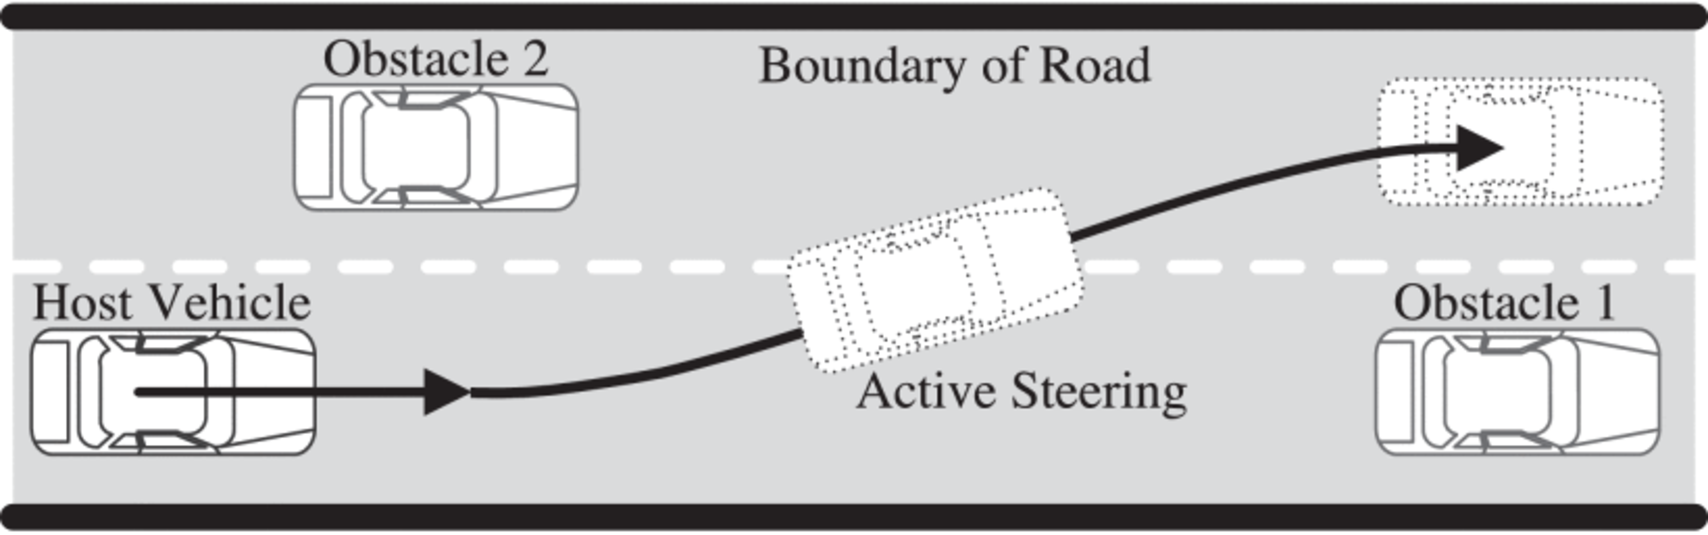
\includegraphics[width=\textwidth]{../figure/obstacleAvoidance/obstacleAvoidance.pdf}
	\caption{Problem description of collision avoidance on a road with only two lanes.}
	\label{fig:obstacleAvoidance}
\end{figure}

The model used in this report should take into account the kinematic and dynamic aspects of the vehicle. Here, we present a non linear mathematical model of a vehicle used for the development of a collision avoidance system.
The model has four states and two inputs:
\begin{equation}
\begin{array}{cc}
\vec{x}=\begin{bmatrix}
x\\y\\\theta\\v 
\end{bmatrix},\qquad 
\vec{u}=\begin{bmatrix}
T\\\delta 
\end{bmatrix}
\end{array} 
\end{equation}
where $(x,y)$ are the global coordinates of the contact point between the rear wheel and the ground, $\theta$ is the heading angle of the car body with respect to the $x$-axis and $v$ is the linear speed of the car (positive). The manipulated variables are $T$ the throttle (positive when accelerating/negative when braking) and $\delta$ the steering angle of the front wheel with respect to the vehicle ($0$ when aligned with car, counterclockwise positive). Figure \ref{fig:car_model} illustrates the applied nonlinear bicycle model and the related parameters.
% BICYCLE MODEL
\begin{figure}[!h]
	\centering
	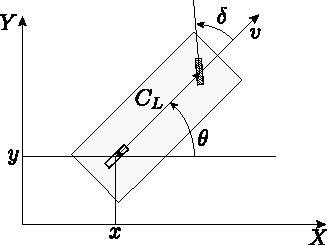
\includegraphics[width=0.80\textwidth]{../figure/car_model.pdf}
	\caption{Bicycle model of a car (adapted from \cite{siciliano}).}
	\label{fig:car_model}
\end{figure}

The ATLASCAR2 can be modeled using the non-linear kinematic bicycle model described by the following equations of motion \cite{safety} \cite{swarms}:
\begin{equation}
\label{eqn:dynamics_model_obstacle_avoidance}
\left \{ \begin{array}{llll}
\dot{x} = v\cos(\theta)\\
\dot{y} = v\sin(\theta)\\
\dot{\theta} =\dfrac{v}{C_L}\tan(\delta)\\
\dot{v} =0.5 \cdot T
\end{array} 
\right .
\Longrightarrow 
\begin{array}{llll}
\dot{\vec{x}} = \vec{f}(\vec{x},\vec{u})\\
\vec{y} = \vec{g}(\vec{x},\vec{u})
\end{array}
\end{equation}
where $C_L$ is the car length. In order to simplify the model, it is assumed that only the front wheel can be steered. Moreover, in this paper it is assumed that the ATLASCAR2 does not slip, so any slippage is thus considered as an external disturbance. Under this assumption, the slip angle is zero, meaning that the velocity is directed along the heading of the vehicle. In order to use MPC, the state space model needs to be linearized with a first order approximation and also re-written in a more compact form:
\begin{equation}
\label{eqn:dynamics_model_non_linear}
\begin{array}{llll}
\dot{\vec{x}} = \vec{f}(\vec{x},\vec{u})\\
\vec{y} = \vec{g}(\vec{x},\vec{u})
\end{array} \Longrightarrow
\begin{array}{ll}
\dot{\vec{x}} =\vec{A}_c \vec{x}+ \vec{B}_c \vec{u}\\
\vec{y} =\vec{C}_c \vec{x} + \vec{D}_c \vec{u}
\end{array}
\end{equation}
where the matrices $\vec{A}_c$, $\vec{B}_c$, $\vec{C}_c$ and $\vec{D}_c$ are obtained as follows:
\begin{equation}
\begin{array}{ccc}
\vec{A}_c=\displaystyle\frac{\partial \vec{f}(\vec{x},\vec{u})}{\partial \vec{x}}=\begin{bmatrix}
0&0&-v\sin(\theta)&\cos(\theta)\\
0&0&v\cos(\theta)&\sin(\theta)\\
0&0&0&\tan(\delta)/C_L\\
0&0&0&0
\end{bmatrix},
\\\\
\vec{B}_c=\displaystyle\frac{\partial \vec{f}(\vec{x},\vec{u})}{\partial \vec{u}}=\begin{bmatrix}
0&0\\
0&0\\
0&\dfrac{v}{C_L}\big(\tan(\delta)^2+1\big)\\
0.5&0
\end{bmatrix},
\\\\
\vec{C}_c=\displaystyle\frac{\partial \vec{g}(\vec{x},\vec{u})}{\partial \vec{u}} = \mathbf{I}_4, 
\qquad
\vec{D}_c=\frac{\partial \vec{g}(\vec{x},\vec{u})}{\partial \vec{u}}=\mathbf{0}_{4\times2}.
\end{array}
\end{equation} 
The simple linearized approximation of the system to describe the dynamics of the ATLASCAR2 will be evaluated at the operating conditions. Note also that the system we are considering is a linear state-space model whose dynamics vary as a function of certain time-varying parameters. The system to be controlled is usually modeled by a discrete state-space model in the MPC literature. Therefore, (\ref{eqn:dynamics_model_non_linear})
is transformed into a discrete state-space model to be used by the Model Predictive Controller:
\begin{equation}
\label{eqn:dynamics_ss_obstacle_avoidance_dis}
\begin{array}{ll}
\dot{\vec{x}} =\vec{A}_c \vec{x}+ \vec{B}_c \vec{u}\\
\vec{y} =\vec{C}_c \vec{x} + \vec{D}_c \vec{u}
\end{array}
\Longrightarrow
\begin{array}{rr}
{\vec{x}}(k+1) =\vec{A}_d \vec{x}(k)+ \vec{B}_d \vec{u}(k)\\
\vec{y}(k) =\vec{C}_d \vec{x}(k) + \vec{D}_d \vec{u}(k)
\end{array}
\end{equation}

where $\vec{A}_d$ and $\vec{B}_d$ are the state and control matrices for the discrete state-space equation, respectively, which can be calculated with the Euler method as
\begin{equation}
\vec{A}_d = e^{\vec{A}_cT_s},\qquad \vec{B}_d = \int_{kT_s}^{(k+1)T_s} e^{\vec{A}_c[(k+1)T_s-\eta]}\vec{B}_c d\eta
\end{equation}

where $T_s$ is the sampling interval for the discrete state-space model. The matrices $\vec{C}_d$ and $\vec{D}_d$ are equivalent to those in the continuous case. For simplicity, we assume that all the states are measurable and the ATLASCAR2 drives east with a constant speed at the nominal operating point. In the scenario that we are going to consider, the road is straight and our vehicle stays in the middle of the center lane when not passing. Without losing generality, the ATLASCAR2 passes an obstacle both to the right and to the left lane depending on where it is placed on the road. We create also a safe zone around the obstacles so that the vehicle does not get too close to the obstacle when passing it.

\section{Design of Adaptive Model Predictive Control}
We designed a Model Predictive Controller that can make the ATLASCAR2 maintain a desired velocity and stay in the middle of center lane. We used an Adaptive MPC controller because it handles the nonlinear vehicle dynamics more effectively than a traditional MPC controller; in fact, the latter uses a constant plant model but the former allows us to provide a new plant model at each control interval. Because the new model describes the plant dynamics more accurately at the new operating condition, an adaptive MPC controller performs better than a traditional MPC controller. In practice, at each control interval, the adaptive MPC controller updates the plant model and the nominal conditions. Once updated, the model and the conditions remain constant over the prediction horizon. In motion planning that uses adaptive MPC, it is common to formulate the constrained control problem as a real-time optimization problem subject to hard constraints on plant variables and soft constraints on outputs; at the beginning, we specified the constraints for the manipulated variables: to prevent the ATLASCAR2 from accelerating or decelerating too quickly, we added an hard constraint on the throttle rate of change and another one on the steering angle rate of change. We used an approach that takes advantage of the ability of MPC to handle constraint explicitly. Figure \ref{fig:flowchart} shows a conditional state machine designed for higher-level behavior planning.

% FLOWCHART
\begin{figure}[!h]
	\centering
	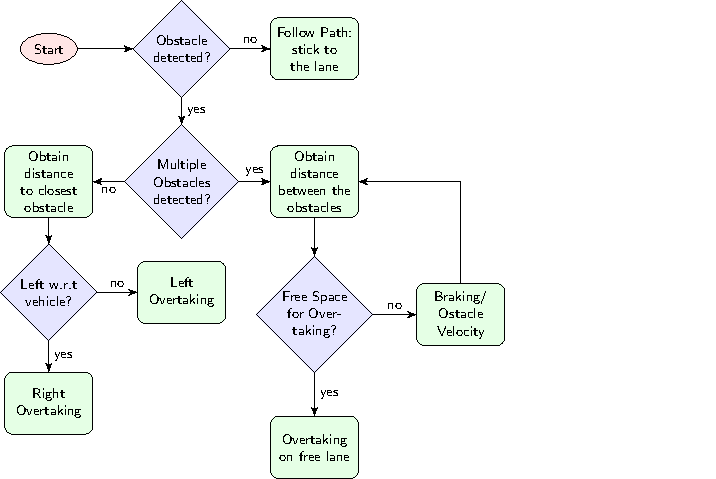
\includegraphics[width=\textwidth]{../figure/flowchart/flowchart.pdf}
	\caption{Behaviour planning conditional flowchart.}
	\label{fig:flowchart}
\end{figure}


When an obstacle is detected, it defines an area on the road (in terms of constraints) that the ATLASCAR2 must not enter during the prediction horizon. At the next control interval the area is redefined based on the new positions of the vehicle and the obstacle until passing is completed.
To define the area to avoid, we used the following mixed Input/Output constraints:
\begin{equation}
\label{eqn:mixed_IO_constraints}
\vec{E}\vec{u}+\vec{F}\vec{y}\leq \vec{G}
\end{equation}
where $\vec{u}$ and $\vec{y}$ are respectively the manipulated variable vector and the output variable vector, while $\vec{E},\vec{F},\vec{G}$ are the constraint matrices that can be updated when the controller is running. Five constraints were defined:
\begin{enumerate}
	\item upper bound on the $y$-coordinate (left boundary of the road);
	\item lower bound on the $y$-coordinate (right boundary of the road);
	\item constraint for obstacle avoidance; although no obstacle is considered in the nominal condition, we must add this virtual constraint here because we cannot change the dimensions of the constraint matrices at run time;
	\item upper bound on the $x$-coordinate (position of the closest obstacle);
	\item lower bound on the $x$-coordinate (position of the ATLASCAR2).
\end{enumerate}
The matrices for the above inequality are the following:
\begin{equation}
\vec{E}= 
\begin{bmatrix}
0&0\\
0&0\\
0&0\\
0&0\\
0&0
\end{bmatrix},
\qquad
\vec{F}=\begin{bmatrix}
0&1&0&0\\
0&-1&0&0\\
cS&-1&0&0\\
1&0&0&0\\
-1&0&0&0\\
\end{bmatrix},
\qquad
\vec{G}=
\begin{bmatrix}
W/2\\W/2\\-cI\\x_{\max}\\x_{\min}
\end{bmatrix}
\end{equation}

where $W$ is the width of the road, $cI$ and $cS$ are the required parameters such that the ATLASCAR2 must be above the line formed from the vehicle to safe zone corner for left/right passing and finally $x_{\max}$ represents the position of the closest obstacle in the case there is not free space for the overtaking (otherwise $x_{\max}=+\infty$) while $x_{\min}$ depicts the location of our vehicle. Figure \ref{fig:constraint} illustrates the constraints that are computed at each $T_s$ in the case of a left overtaking.
% FIGURE CONSTRAINT
\begin{figure}[!h]
	\centering
	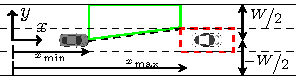
\includegraphics[width=\textwidth]{../figure/constraint/constraint.pdf}
	\caption{Constraints in the case of left overtaking.}
	\label{fig:constraint}
\end{figure}

\section{Simulation Results}
The performances of the proposed adaptive MPC based vehicle control method are demonstrated in three simulation examples. We tried to choose parameters that were as close as possible to a real situation: the sampling time used in the discretization of the system is $T_s=\SI{0.02}{s}$ while the values of the prediction and the control horizon are respectively $p_H=25$ and $c_H=5$. In all simulations, the distance between the front and rear axles is $C_L=\SI{5}{m}$ and the width of the vehicle is $C_W=\SI{2}{m}$. The saturation ranges of the control inputs are: the steering angle lies in $\big[-\frac{\pi}{30}, +\frac{\pi}{30}\big]$ rad/s while in order to prevent the ATLASCAR2 from accelerating or decelerating too quickly, we impose an hard constraint of \SI{2.5}{m/s^2} on the throttle rate of change. Moreover we are using a constant reference signal for the velocity of $v=\SI{20}{m/s}$ ($\approx\SI{72}{km/h}$).
Blue paths in Figures \ref{fig:obstacleAvoidance_one_obstacle}, \ref{fig:obstacleAvoidance_random}, \ref{fig:braking} are known only at the end of the simulations.

\subsection{One Moving Obstacle - Right Overtaking}
In this first simulation
(Figure \ref{fig:obstacleAvoidance_one_obstacle}) the ATLASCAR2 drives in the middle of the center lane while the road is completely free and when there is an obstacle, the vehicle passes it only using the right lane (the same simulation can be launched so that the car goes over to the left fast lane). In other words if the ATLASCAR2 is already in the adjacent lane, it uses the safety zone as the constraint, otherwise the vehicle must be above the line formed from the ATLASCAR2 to safe zone corner for right passing. If the vehicle is parallel to the obstacle, it  uses the safety zone as the constraint and finally if it has passed the obstacle, it uses the inactive constraint to go back to the center lane.
Algorithm \ref{alg:rightOvertaking} summarizes the main steps to compute custom constraints for the obstacle; when the vehicle detects the obstacle, the constraints are computed. In this simulation only the first three constraints are necessary because there is space for the overtaking without braking (the fourth and fifth constraints don't change).

% ONE MOVING OBSTACLE
\begin{figure}[h!]
	\centering
	\begin{minipage}[t]{\textwidth}
		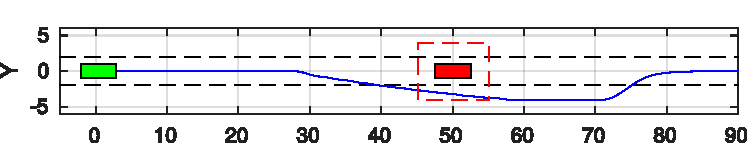
\includegraphics[width=\textwidth]{../figure/one_obstacle_right_overtaking/overtaking_start.pdf}
	\end{minipage}
	\begin{minipage}[t]{\textwidth}
		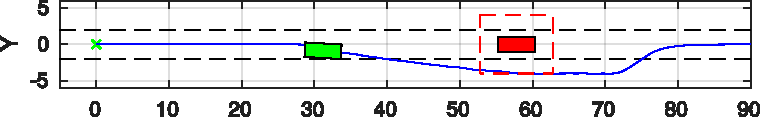
\includegraphics[width=\textwidth]{../figure/one_obstacle_right_overtaking/overtaking_middle.pdf}
	\end{minipage}
	\begin{minipage}[t]{\textwidth}
		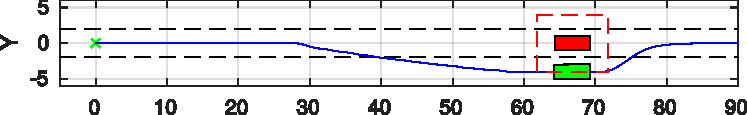
\includegraphics[width=\textwidth]{../figure/one_obstacle_right_overtaking/overtaking_middle_end.pdf}
	\end{minipage}
	\begin{minipage}[t]{\textwidth}
		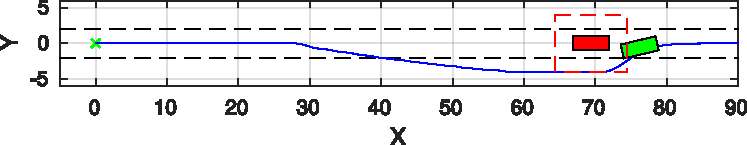
\includegraphics[width=\textwidth]{../figure/one_obstacle_right_overtaking/overtaking_end.pdf}
	\end{minipage}
	\caption{Simulation of right overtaking with one moving obstacle that moves in the same direction as the vehicle.}
	\label{fig:obstacleAvoidance_one_obstacle}
\end{figure}

% ALGORITHM FOR RIGHT OVERTAKING OF ONE MOVING OBSTACLE
\begin{algorithm}%[b]
	\caption{Right Overtaking if an obstacle is detected}
	\small
	\begin{algorithmic}[1]
		\Function{RightOvertaking}{car, obstacle, road}
		\State $x_\text{min} \gets \text{car}X $,  $x_\text{max} \gets +\infty$;
		\State obsYrr = obstacle.RearRightSafeY;
		\State obsXrr = obstacle.RearRightSafeX;
		\If{ATLASCAR2 is behind the obstacle} 
		\If{ATLASCAR2 is in the adjacent lane}
		\State $cS \gets 0$; $cI \gets \text{obsYrr}$;
		\Else
		\State $cS \gets \text{tan}(\text{atan2}(\frac{\text{obsYrr}-\text{ carY}}{\text{obsXrr}-\text{carX}},1))$;
		\State $cI \gets \text{obsYrr}-cS*\text{obsXrr}$;
		\EndIf
		\Else
		\If{ATLASCAR2 is parallel to the obstacle}
		\State $cS \gets 0$; $cI \gets \text{obsYrr}$;
		\Else
		\State $cS \gets 0$; $cI \gets W/2$;
		\EndIf
		\EndIf
		\State \Return $x_\text{min}$, $x_\text{max}$, $cI$, $cS$
		\EndFunction
	\end{algorithmic}
	\label{alg:rightOvertaking}
\end{algorithm}

% OVERALL SCHEME ONE MOVING OBSTACLE
\begin{figure}[!h]
	\centering
	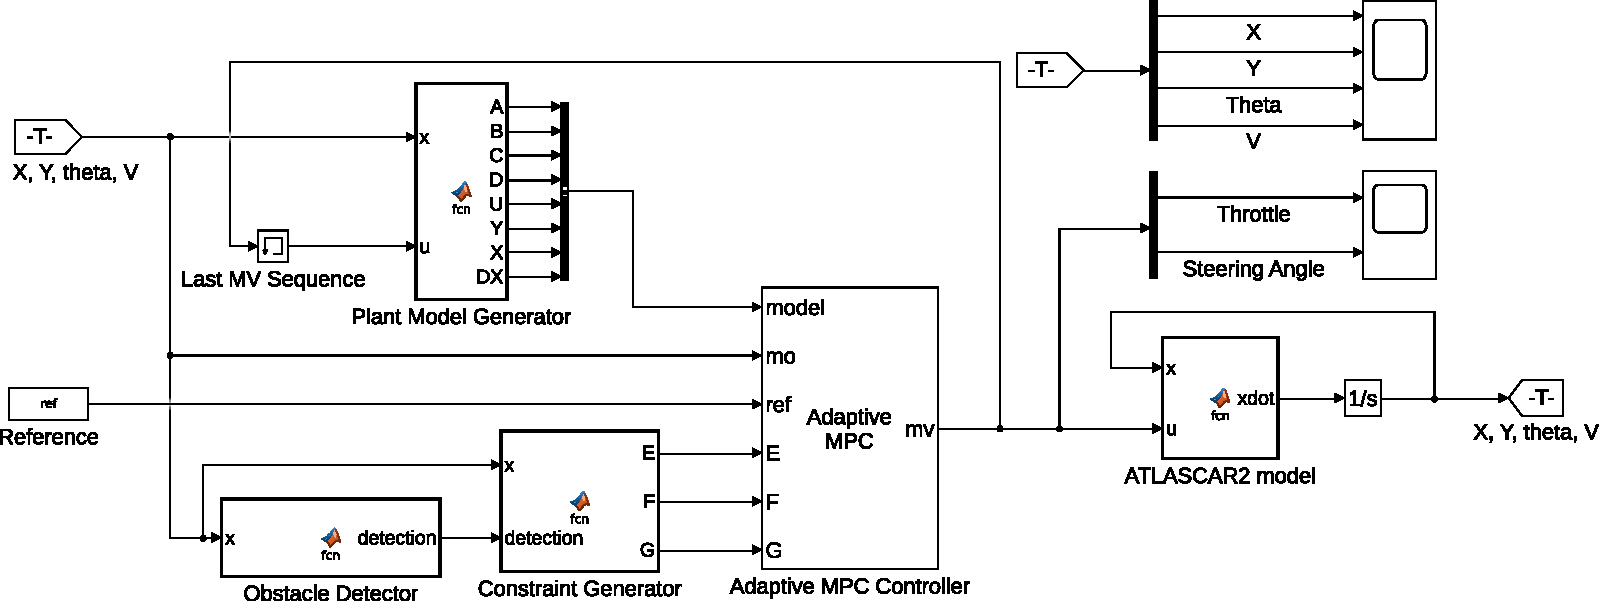
\includegraphics[width=\textwidth]{../figure/MovingObstacleAvoidance.pdf}
	\caption{Overall procedure scheme moving obstacle avoidance.}
	\label{fig:MovingObstacleAvoidance}
\end{figure}
%
\subsection{Multiple Moving Obstacles}
For a second test, additional obstacles were added to make the scenario more complex (Figure \ref{fig:obstacleAvoidance_random}).
% MULTIPLE MOVING OBSTACLE
\begin{figure}[!h]
	\centering
	\begin{minipage}[t]{\textwidth}
		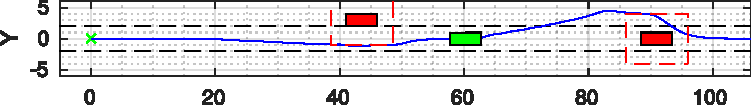
\includegraphics[width=\textwidth]{./figure/random_N_obstacles/overtaking_random_2.pdf}
	\end{minipage}
	\begin{minipage}[t]{\textwidth}
		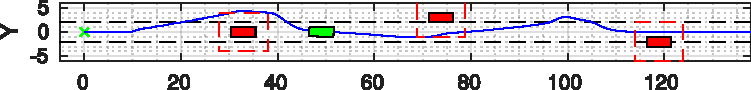
\includegraphics[width=\textwidth]{./figure/random_N_obstacles/overtaking_random.pdf}
	\end{minipage}
	\begin{minipage}[t]{\textwidth}
		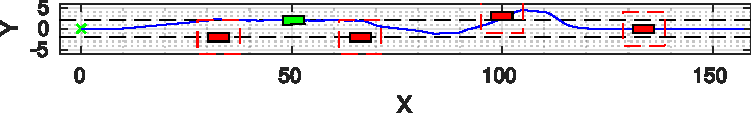
\includegraphics[width=\textwidth]{./figure/random_N_obstacles/overtaking_random_1.pdf}
	\end{minipage}
	\caption{Simulations of overtaking with $N = 2,3,4$ moving obstacles that drive in the opposite direction with respect to the ATLASCAR2.}
	\label{fig:obstacleAvoidance_random}
\end{figure}

The vehicle is capable of overtaking the obstacles on the right or left depending on their positions with respect to the road. If the $y$-coordinate of the closest obstacle is greater than 0, then the vehicle overtakes to the right, otherwise the overtaking takes place on the left lane. We also hypothesized that the obstacles move at different speeds but that they are initially at a common distance; they can have a uniform motion or a uniformely accelerated motion. In case two obstacles are too close during the simulation and their distance is less than the detection range, which is \SI{30}{m}, the ATLASCAR2 perceives the objects as a single entity and adapts to the situation. The same test can be done with the obstacles that drive in the same direction as the vehicle but to better assess and demonstrate results we decided to show a very unusual scenario.

\subsection{Vehicle Braking and Obstacles Overtaking}
Finally we have improved the code related to the mixed Input/Output constraints so that in the case there are 3 obstacles that block the road and drive at a lower speed than the ATLASCAR2, the velocity of the vehicle decreases in order to prevent the collision. Figure \ref{fig:braking} depicts a simulation in which there are 3 obstacles at the same $x$-coordinate. Two obstacles have a constant speed of \SI{8}{m/s} while the one on the left lane of \SI{15}{m/s}.
In this particular case it is essential to consider the fourth and the fifth restriction in order to allow the ATLASCAR2 to slow down without colliding with the cars in front. The fifth constraint is simply the position of the ATLASCAR2 that updates at each interval, while the fourth constraint, until there is a free lane, is the position of the closest obstacle (both the positions are with respect to the global reference frame). In the calculation of the fourth constraint is necessary  to consider the speed at which the vehicle and the obstacle are moving in order to keep a safe distance. In particular three parameters have been identified as the key
factors computing the safe distance between cars:
\begin{itemize}
	\item detection range of the ATLASCAR2;
	\item velocities of the vehicle and the obstacle;
	\item distance between the cars.
\end{itemize}

% BRAKING THREE OBSTACLE
\begin{figure}[!h]
	\centering
	\begin{minipage}[t]{\textwidth}
		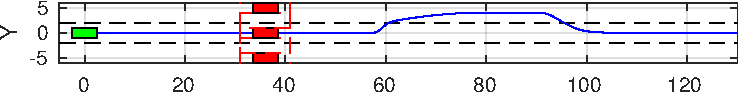
\includegraphics[width=\textwidth]{./figure/three_obstacles_no_overtaking/braking_0.pdf}
	\end{minipage}
	\begin{minipage}[t]{\textwidth}
		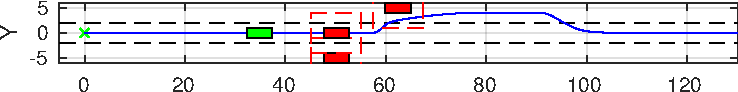
\includegraphics[width=\textwidth]{./figure/three_obstacles_no_overtaking/braking_1.pdf}
	\end{minipage}
	\begin{minipage}[t]{\textwidth}
		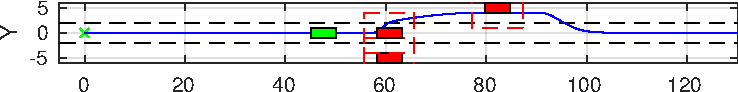
\includegraphics[width=\textwidth]{./figure/three_obstacles_no_overtaking/braking_2.pdf}
	\end{minipage}
	\begin{minipage}[t]{\textwidth}
		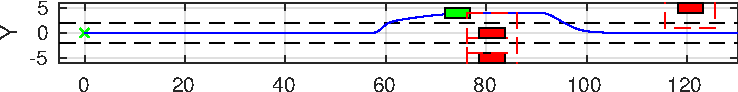
\includegraphics[width=\textwidth]{./figure/three_obstacles_no_overtaking/braking_3.pdf}
	\end{minipage}
	\begin{minipage}[t]{\textwidth}
		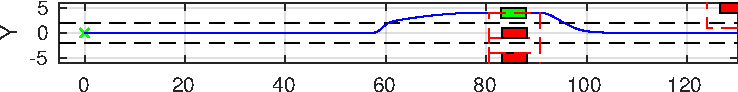
\includegraphics[width=\textwidth]{./figure/three_obstacles_no_overtaking/braking_4.pdf}
	\end{minipage}
	\begin{minipage}[t]{\textwidth}
		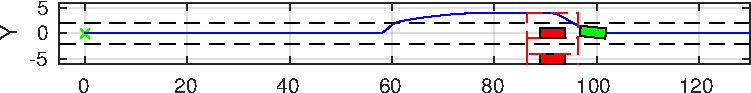
\includegraphics[width=\textwidth]{./figure/three_obstacles_no_overtaking/braking_5.pdf}
	\end{minipage}
	\begin{minipage}[t]{\textwidth}
		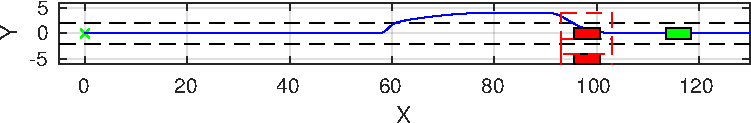
\includegraphics[width=\textwidth]{./figure/three_obstacles_no_overtaking/braking_6.pdf}
	\end{minipage}
	\caption{Simulation of braking and overtaking obstacles.}
	\label{fig:braking}
\end{figure}

At the beginning, the vehicle moves with the reference velocity of $v=\SI{20}{m/s}$. When the ATLASCAR2 detects all the other cars on the road, checks if there is a free lane. In the first part of the simulation, the ATLASCAR2 brakes because there is not enough space for overtaking the cars as shown in Fig. \ref{fig:velocity_braking}. A collision would happen if the vehicle continues to follow the initially planned path with the reference velocity. It is possible to notice that the speed decreases because the applied throttle is negative, so a consistent deceleration is set after $\approx\SI{1.5}{s}$ as depicted in Fig. \ref{fig:throttle_braking}. The velocity of the ATLASCAR2 for $\approx\SI{2}{s}$ adapts to that of the closest obstacle. After a few seconds the fastest car moves and makes available the left lane for overtaking. Dramatic changes of steering angle in early stage are observed in Fig. \ref{fig:delta_braking} and consequently also on the heading angle in Fig. \ref{fig:theta_braking}. Then, the ATLASCAR2 returns to the reference velocity during the overtaking of the two obstacles (the applied throttle after $\approx\SI{5}{s}$ is positive). It is seen that the ATLASCAR2 avoids the obstacles and returns to the road center line with a low overshoot.

% RESULTS BRAKING THREE OBSTACLES
\begin{figure}[!t] %vs changes to t instead of b
	\begin{minipage}[t]{0.5\textwidth}
		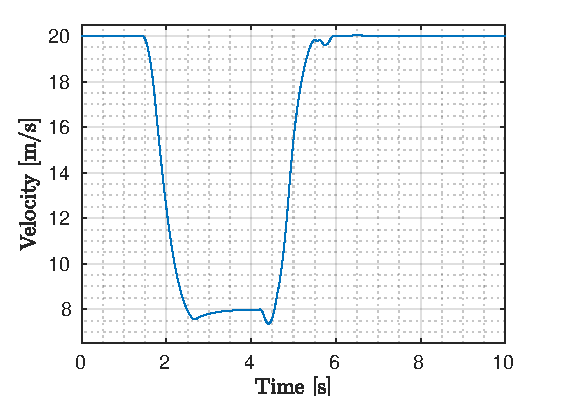
\includegraphics[width=\textwidth]{./figure/three_obstacles_no_overtaking/VelocityVsTime.pdf}
		\subcaption{}\label{fig:velocity_braking}
	\end{minipage}
	\begin{minipage}[t]{0.5\textwidth}
		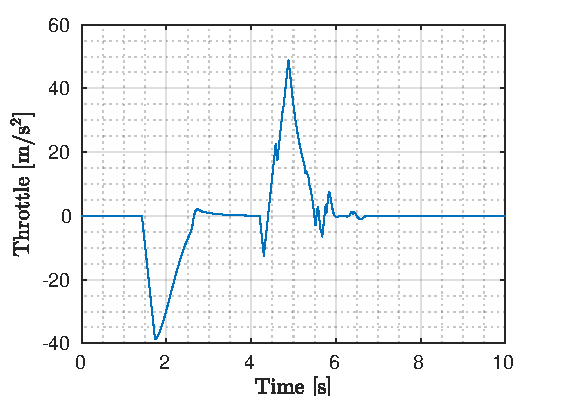
\includegraphics[width=\textwidth]{./figure/three_obstacles_no_overtaking/ThrottleVsTime.pdf}
		\subcaption{}\label{fig:throttle_braking}
	\end{minipage}
	\begin{minipage}[t]{0.5\textwidth}
		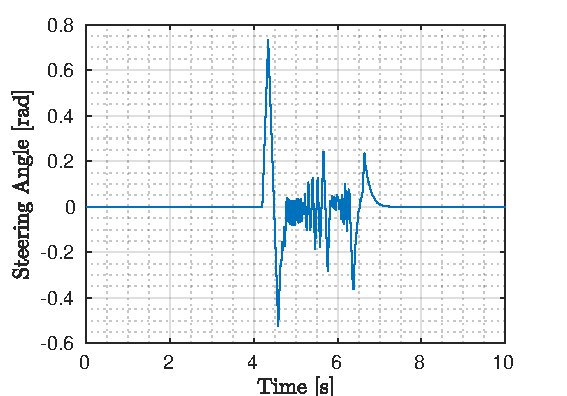
\includegraphics[width=\textwidth]{./figure/three_obstacles_no_overtaking/SteeringAngleVsTime.pdf}
		\subcaption{}\label{fig:delta_braking}
	\end{minipage}
	\begin{minipage}[t]{0.5\textwidth}
		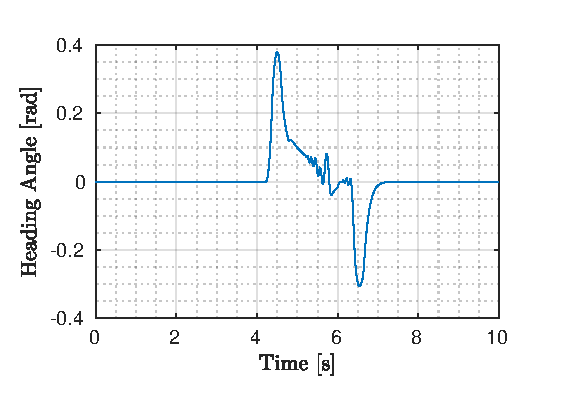
\includegraphics[width=\textwidth]{./figure/three_obstacles_no_overtaking/HeadingAngleVsTime.pdf}
		\subcaption{}\label{fig:theta_braking}
	\end{minipage}
	\caption{Time signals of the ATLASCAR2 in the simulation of braking and overtaking in the situation illustrated in Figure \ref{fig:braking}.}
	\label{fig:components}
\end{figure}

\cleardoublepage
\chapter{Chapter 6}

\cleardoublepage
\chapter*{Conclusions and Future Work}
\addcontentsline{toc}{chapter}{Conclusions and Future Work}
\setstretch{\dnormalspacing}

% the back matter
%\backmatter

 \clearpage
 \bibliography{references}
 \addcontentsline{toc}{chapter}{References}
 \bibliographystyle{ieeetr}

% \include{endmatter/colophon}

\end{document}
